%
% Modified by Megan Patnott
% Last Change: Jan 18, 2013
%
%%%%%%%%%%%%%%%%%%%%%%%%%%%%%%%%%%%%%%%%%%%%%%%%%%%%%%%%%%%%%%%%%%%%%%%%
%
% Modified by Sameer Vijay
% Last Change: Tue Jul 26 2005 13:00 CEST
%
%%%%%%%%%%%%%%%%%%%%%%%%%%%%%%%%%%%%%%%%%%%%%%%%%%%%%%%%%%%%%%%%%%%%%%%%
%
% Sample Notre Dame Thesis/Dissertation
% Using Donald Peterson's ndthesis classfile
%
% Written by Jeff Squyres and Don Peterson
%
% Provided by the Information Technology Committee of
%   the Graduate Student Union
%   http://www.gsu.nd.edu/
%
% Nothing in this document is serious except the format.  :-)
%
% If you have any suggestions, comments, questions, please send e-mail
% to: ndthesis@gsu.nd.edu
%
%%%%%%%%%%%%%%%%%%%%%%%%%%%%%%%%%%%%%%%%%%%%%%%%%%%%%%%%%%%%%%%%%%%%%%%%


%
% Chapter 4
%


\chapter{Lifetime Measurements}
\label{chap: lifetime}

This chapter presents the details of the analysis used for the determination of the lifetime of the 6.79 MeV state, the 5.18 MeV state, and the 6.17 MeV state in $^{15}$O. These data resulted from a nine-day long experiment at the university of Notre Dame Nuclear Science Laboratory in August 2019. This measurement used protons from the 5U Sta. Ana accelerator for the $^{14}$N(p,$\gamma$)$^{15}$O reaction at beam energies ranging from 1 MeV to 1.6 MeV. Further description of this experimental setup, targets, and methodology can be found in Chapter \ref{chap: experiment}.	

\section{Determining a nuclear lifetime}
\label{sec: lifetime determination}

For this analysis, a new DSAM program was written to simulate the expected Doppler shift and lineshape. This approach, as will be outlined shortly, follows the Monte Carlo (MC) technique for simulating physical phenomena with the sampling of random numbers. A full reproduction of the code is provided for reference in Appendix \ref{appendix: codes}. 

The MC technique is simple enough in idea and a powerful tool across the fields of physics and mathematics: to numerically estimate phenomena by studying their effects with reasonably sampled, random numbers. In other words, the aim is to build a probability distribution that is proportional to some function, $P(x)$, which spans the interval $[x_{min}, x_{max}]$, using random numbers in the range [0,1]. To start, take the integral of the function over some subset of its total range,

\begin{equation}
I(x) = \int_{x_{min}}^{x} P(x') dx',
\label{eqn: mcStart}
\end{equation}

\noindent where $x_{min} \leq x \leq x_{max}$. Normalizing this integral to the integral over the complete range,

\begin{equation}
I_{norm}(x) = \dfrac{I(x)}{I(x_{max})} = \dfrac{\int_{x_{min}}^{x} P(x') dx'}{\int_{x_{min}}^{x_{max}} P(x') dx'},
\end{equation}

\noindent creates the desired relationship, since the integrated probability is itself a random variable and the normalization guarantees its range is confined to [0, 1]. This is shown when evaluating $I_{norm}$ at the extremes of its domain,

\begin{equation}
I_{norm} (x_{min}) = \dfrac{\int_{x_{min}}^{x_{min}} P(x') dx'}{\int_{x_{min}}^{x_{max}} P(x') dx'} = 0
\end{equation}

\noindent and

\begin{equation}
I_{norm} (x_{max}) = \dfrac{\int_{x_{min}}^{x_{max}} P(x') dx'}{\int_{x_{min}}^{x_{max}} P(x') dx'} = 1.
\end{equation}

\noindent Finally, then, to utilize this relationship in the MC technique, $I_{norm}$ is evaluated for a specific function and ultimately inverted to produce a response in the original function, $P(x)$, as a function of a randomly generated number in the range of [0, 1].

Specifically, the case of interest in this work involves the modeling of exponential decay,

\begin{equation}
P(x) = e^{-\lambda x},
\end{equation}

\noindent where $\lambda$ is the width and inversely proportional to the lifetime, $\lambda = 1/ \tau$. In this context, the domain of input variable, $x$, is [0, $\infty$], as the decay can occur at any time. Utilizing this in the formulation starting with Equation \ref{eqn: mcStart},

\begin{equation}
I(x) = \int_{0}^{x} e^{-\lambda x'} dx' = \frac{1}{\lambda} (1 - e^{-\lambda x}),
\end{equation}

\begin{equation}
I(x_{min}) = I(0) = 0,
\end{equation}

\begin{equation}
I(x_{max}) = I(\infty) = 1/\lambda,
\end{equation}

\noindent and, ultimately, 

\begin{equation}
I_{norm}(x) = \frac{\lambda^{-1}(1 - e^{-\lambda x})}{\lambda^{-1}} = (1 - e^{-\lambda x}).
\label{eqn: exponentialGenerator}
\end{equation}

\noindent An example of this approach is plotted for reference in Fig.\ \ref{fig: expoGen}. This plots Equation \ref{eqn: exponentialGenerator} for the arbitrary choice of $\lambda$=50 to demonstrate the operational principles. The range of this function's response is limited to [0, 1], as it approaches 1 asymptotically. While the input variable, decay time, is only plotted to 0.1 in this figure, the behavior does not change at higher values and was only chosen to highlight this method. Now, a random number, $r$, can be generated on the range [0, 1], i.e.\ within the range of $I_{norm}(x)$, and this curve can be used to look up and identify a value for the specific decay time, $x$. 



\begin{figure}
\thisfloatpagestyle{plain}
\centering
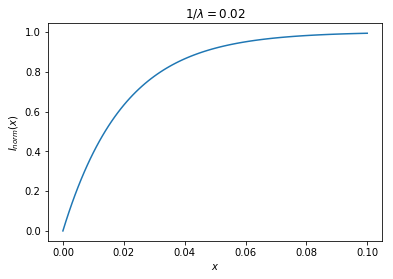
\includegraphics[width=0.85\linewidth]{figures/expoDecayGenerator.png}
\caption{An example of the Monte Carlo method for constructing a relationship between a function and the random number generator. This plots the $I_{norm}(x)$ of Equation \ref{eqn: exponentialGenerator} for an arbitrary choice of $\lambda = 50$ to demonstrate the technique. The range of the response of this function is limited to [0, 1] asymptotically, while the input variable of decay time is unrestricted. }
\label{fig: expoGen}
\end{figure}


However, this can be more instructive to invert the function and create a relationship to output a decay time for a randomly generated $r$ and a given width and lifetime, $\lambda$ and $\tau$, respectively.  This is done as,

\begin{equation}
r = 1 - e^{-\lambda x} \Rightarrow e^{\lambda x} = \dfrac{1}{1-r} \Rightarrow x = \dfrac{1}{\lambda} \ln \left( \frac{1}{1-r} \right).
\label{eqn: rand}
\end{equation}

\noindent The above relationship is then used to simulate a decaying nucleus. By selecting a random number within [0, 1] one can determine the corresponding decay time of a nucleus with a given lifetime from Equation \ref{eqn: rand}. For a large amount of randomly generated numbers, the general behavior of the initial function, exponential decay in this case, can be simulated and studied. An example of this is shown in Fig.\ \ref{fig: simExample} for 100,000 such events. The total behavior can be stored and compared with the original decay law. To do this, however, the simulated histogram must be normalized to match the properties of the original function, $P(x)$.  Namely, the survival cannot be greater than 1, and, indeed, $P(0) = 1$. Therefore, by normalizing the whole histogram to the value of the first histogram bin, the simulated decay curve can be compared to the function from which it was generated. As Fig.\ \ref{fig: simCompare} demonstrates, this is a effective and faithful method of simulating these natural phenomena. 


\begin{figure}
\centering
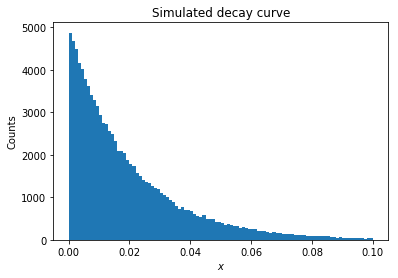
\includegraphics[width=0.85\linewidth]{figures/simExample.png}
\caption{An example of the Monte Carlo method for a simulated decay curve. For 100,000 simulated nuclear decays with a $\lambda$=50, the MC method generates the given histogram of decay times.  }
\label{fig: simExample}
\end{figure}


\begin{figure}
\thisfloatpagestyle{plain}
\centering
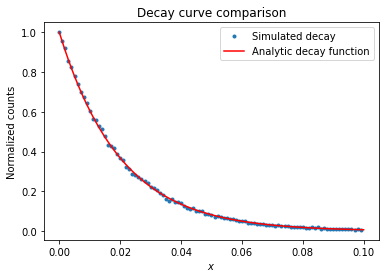
\includegraphics[width=\linewidth]{figures/simCompareExample.png}
\caption{An example of the Monte Carlo method for a simulated decay curve. For 100,000 simulated nuclear decays with a $\lambda$=50, the MC method generates the given histogram of decay times.  }
\label{fig: simCompare}
\end{figure}


It is upon these principles and this derived formulation that the experimentally measured nuclear lifetimes were extracted. A full reproduction of the code is provided for reference in Appendix \ref{appendix: codes}. The important components of the code are illustrated in Fig.\ \ref{fig: simSteps} and the logic of the code is as follows:


\begin{figure}
\thisfloatpagestyle{plain}
\centering
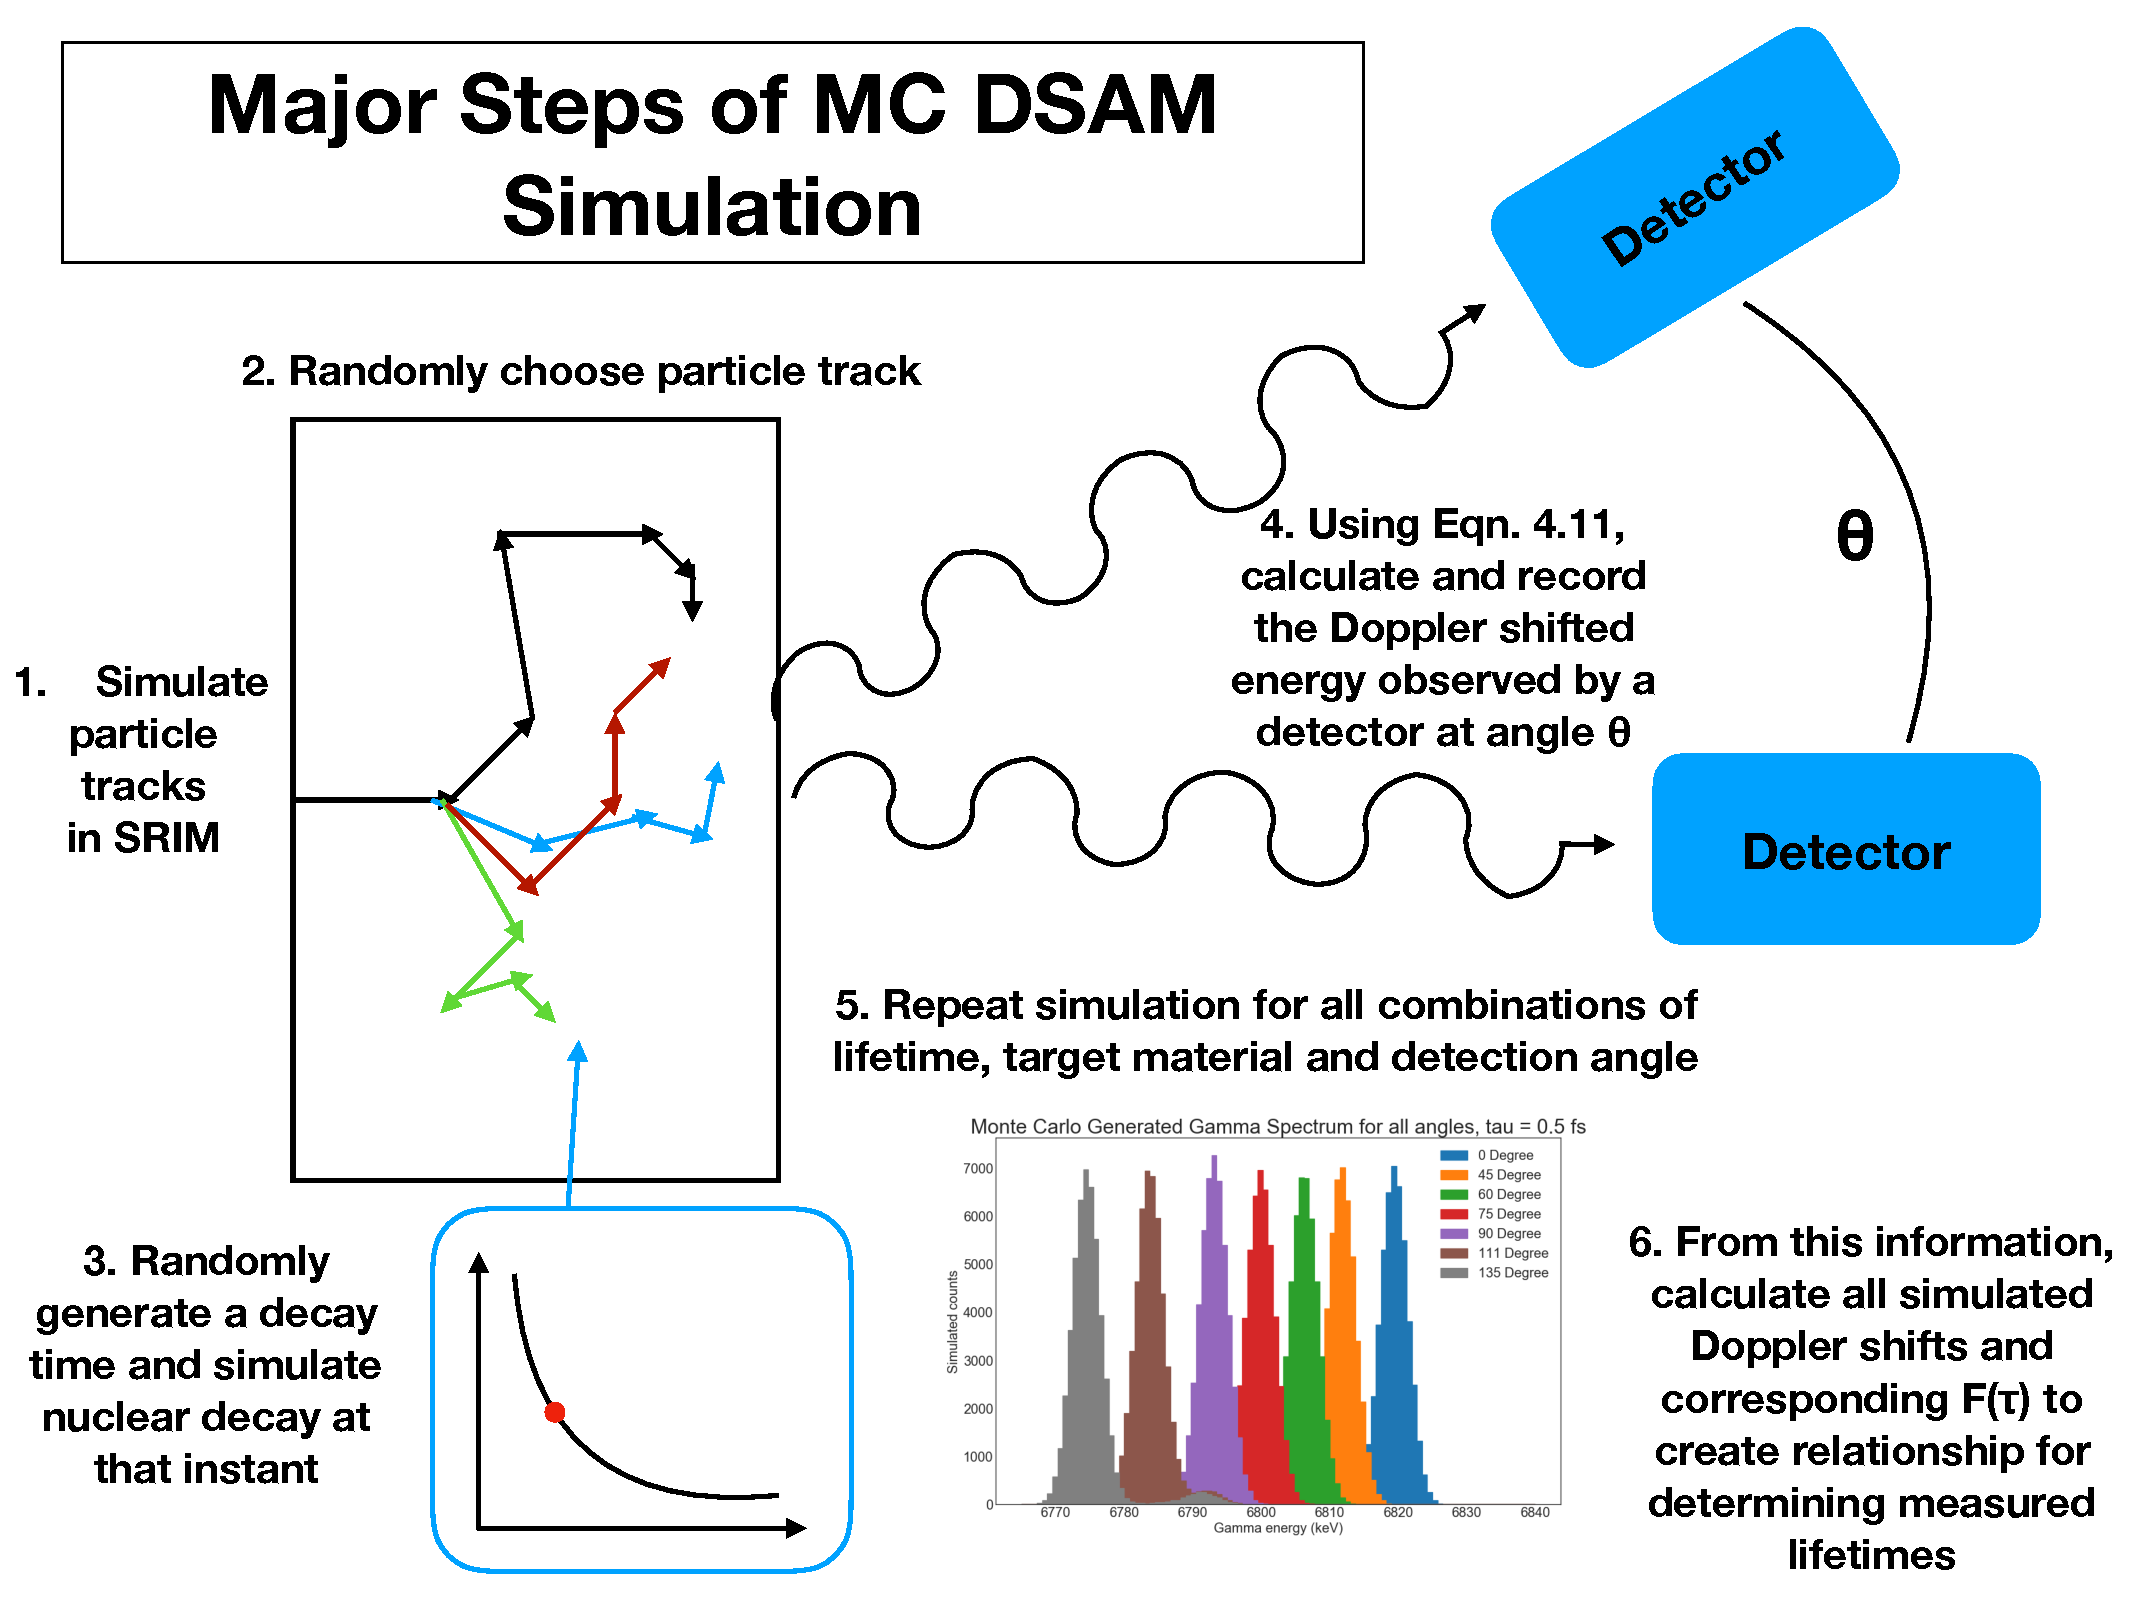
\includegraphics[width=\linewidth]{figures/simSteps.pdf}
\caption{The major steps of the Monte Carlo DSAM simulation for each $\gamma$ ray event. The details of the process are provided in the text, with a complete reproduction of the code also included in Appendix \ref{appendix: codes}.}
\label{fig: simSteps}
\end{figure}


\begin{enumerate}
\item First, recoil ion travel paths were calculated with the SRIM software \cite{Ziegler2010} (another Monte Carlo simulation) for each target material, accounting for the nitrogen present. For this, the reaction recoil energy was calculated and used as the input energy of the ion. The initial energy was randomly assigned to a reasonable range based on the energy loss in the target before reaching the implanted depth of nitrogen. All recoils were assumed to have initial velocity parallel to the incident beam axis. Then, the software calculates the path of the ions travel, recording the the ion's energy, the location of each collision, and the stopping power felt at that position. These tracks are randomly generated for 10,000 different ions. The standard SRIM output is sufficient in this case as the energy regime for this reaction is not high enough to warrant relativistic corrections, like the methods of \cite{Galinski2014, Michelagnoli2013}. 
\item Next, based on the information from the SRIM output, further information about each ion's travel is calculated. Specifically, utilizing the position of each interaction, the particle's trajectory is calculated between each collision. Using the ion's energy at each point, the speed is calculated. Then, ultimately using these data, the time for each interaction (in femtoseconds) is determined. This provides a complete picture of any single ion's calculated motion through the target material. As these are not relativistic quantities, standard freshman kinematics relations are all that is necessary to calculate this information.
\item Of the 10,000 tracks for which the information has been calculated, randomly select one to be the specific decaying ion's path. 
\item Choose a specific nuclear lifetime for the decaying nuclear state to simulate and angle of detection. The angles chosen to simulate were the same as the angles used in the measurement for a direct comparison. 
\item Using the relationship in Equation \ref{eqn: rand} and the specified nuclear lifetime from the previous step, randomly generate a decay time for the recoiling nucleus.  
\item At the given, generated decay time, the code looks up the calculated information for the previous and subsequent collisions. From these, it interpolates between the two interactions to find the position and velocity of the decaying nucleus. 
\item Calculate, explicitly, the Doppler shifted energy, $E_{\gamma}$, from a nucleus decaying at this time, with a specified velocity, $\beta = v/c$, and with the gamma being observed by a detector at a specified angle, $\theta$,

\begin{equation}
E_{\gamma} = E_{\gamma}^{0} ( 1 + \beta \cos (\theta)) \times R
\label{eqn: doppSim}
\end{equation}

\noindent where $R$ represents a correction to account for the detector size and resolution, determined from the experimental spectra, and $E_{\gamma}^{0}$ is the unshifted $\gamma$ ray energy. At this point, it is important to note that as this measurement was not intended to calculate a cross-section, the detection efficiency is not included in this simulation. 
\item The code then records the energy of this measured $\gamma$-ray and adds it to a histogram for it's specific decay time, measured angle, and target material. This behavior is illustrated in Fig.\ \ref{fig: simulatedSingle}, which shows the simulated energy deposition histograms at each of the angles.

\begin{figure}
\thisfloatpagestyle{plain}
\centering
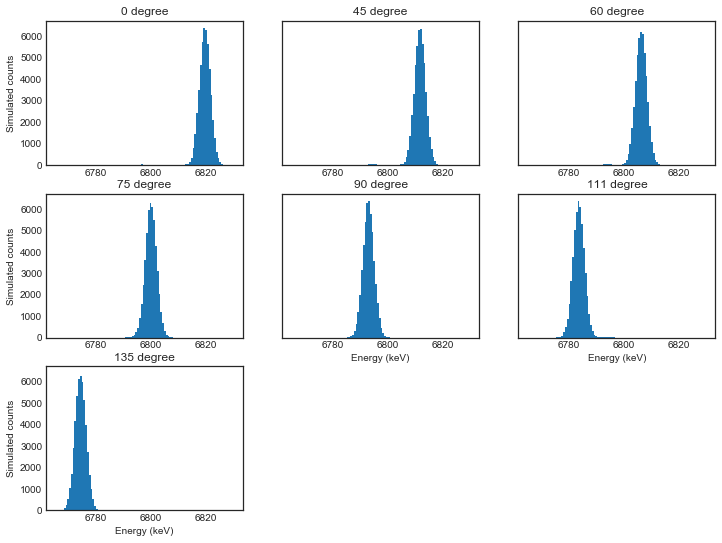
\includegraphics[width=\linewidth]{figures/simulatedSingle.png}
\caption{Simulated energy deposition histograms for the Mo target implantation material with a nuclear lifetime of $\tau=0.5$ fs from the decay of the 6792 keV state in $^{15}$O. Each histogram represents the detection of the 50,000 of the decaying $\gamma$-rays at the angle specified. As all the histograms share common axis bounds, the Doppler shift with angle can clearly be seen. The plot for 0 degree shows the maximum shifted gamma ray, where the unshifted photons arrive at 6792 keV in the 90 degree histogram, matching the real data. A plot of all shifts together is shown later, in Fig.\ \ref{fig: simulatedAll}. The shifting down of the peak with respect to angle shows the Doppler Shift in action.}
\label{fig: simulatedSingle}
\end{figure}

\item The code then returns to Step 3 and repeats this simulation for 50,000 decays for each detection angle, lifetime, and target material combination. An even clearer example of the Doppler shift within this MC simulation is presented in Fig.\ \ref{fig: simulatedAll}. This presents one specific lifetime, $\tau=0.5$ fs, with the Mo backing to show all the simulated $\gamma$'s on one plot. This shows the boost in energy at forward angles ($\theta < 90 \degree$) and the reduction in energy at backward angles ($\theta > 90 \degree$). 


\begin{figure}
\thisfloatpagestyle{plain}
\centering
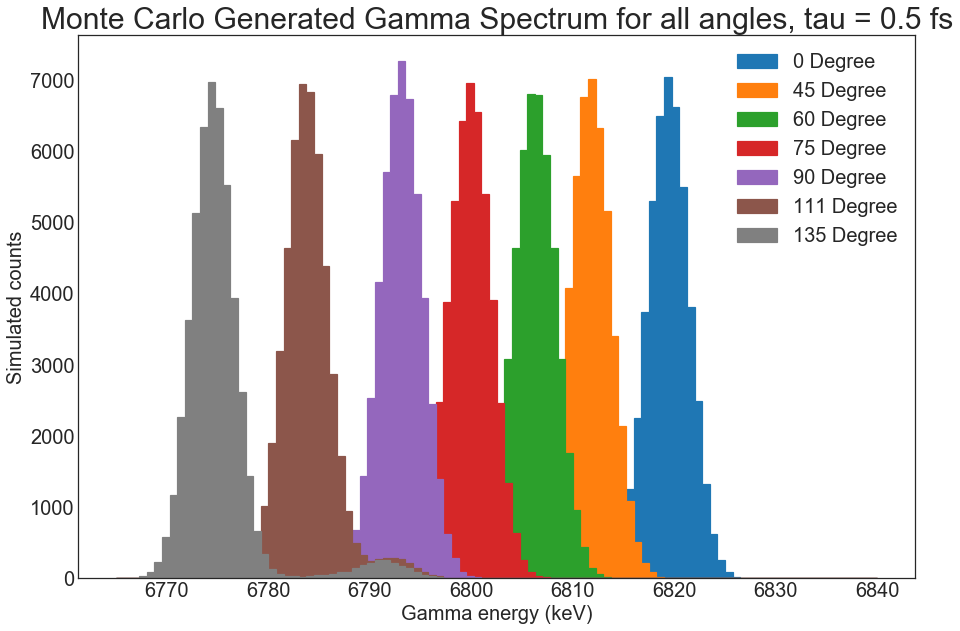
\includegraphics[width=\linewidth]{figures/simAllAngles.png}
\caption{Simulated energy deposition histogram for all detection angles. This plot was produced from the decay of $^{15}$O through the 6.79 MeV state with the Mo backing material and lifetime $\tau=0.5$ fs, where each color represents a different detection angle. Clearly illustrated in this figure is the Doppler shift of the $\gamma$ ray energies with changing angle, the relationship upon which the entire DSA method is predicated. After each peak in this figure is fit with a Gaussian, the centroids were used to determine the energy shift as a function of angle. Under these simulated conditions, the maximum shift is roughly 26 keV. The unshifted photons are also detected at 6792 keV, exactly matching experimental conditions.}
\label{fig: simulatedAll}
\end{figure}


\item These aggregate histograms are all used to determine the peak locations since they are the shifted peaks. This establishes the direct link between the gamma's energy and angle. Therefore, the relationship between shifted $\gamma$ ray energy at each of the conditions for lifetime, angle, and material is determined in this way. 
\item At this point, takes all of this information from each combination to plot a relationship between the observed energy in the detector vs. $\cos(\theta)$, as is done in the experiment. Each is fit with a line, the slope of which contains the attenuation factor information. An example of this process is illustrated in Fig.\ \ref{fig: simSlopes}, showing all of the combinations of lifetime and angle for the Mo target simulations.

\begin{landscape}
\begin{figure}
\thisfloatpagestyle{plain}
\centering
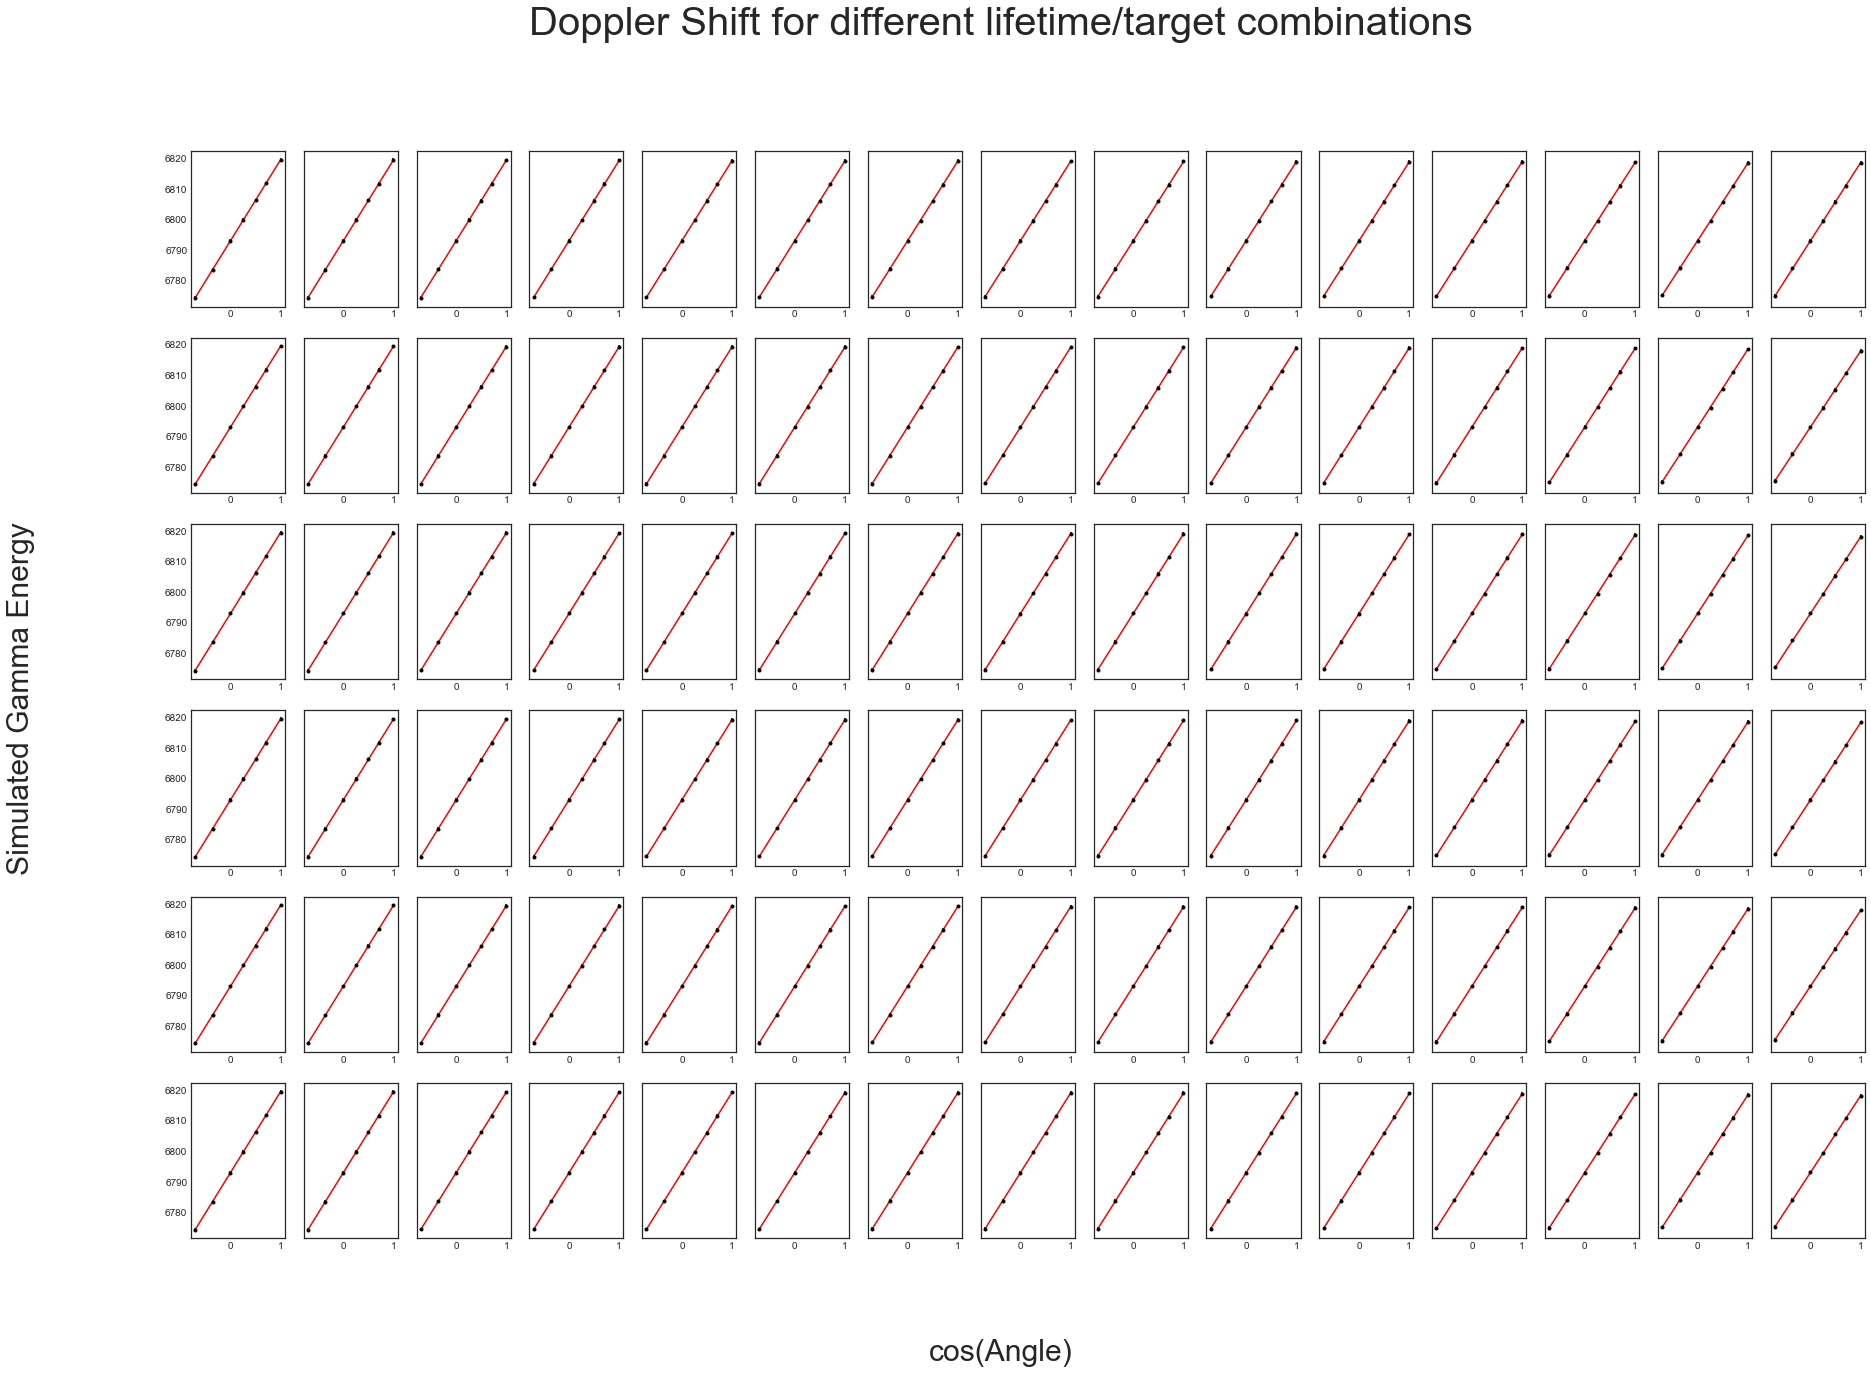
\includegraphics[width=0.7\linewidth]{figures/simSlopes.png}
\caption{Determining the relationship between shifted peak energy and $\cos(\theta)$ for all simulated Mo lifetime combinations. This provides the output of the slopes for each simulated condition, allowing one to establish a relationship between the slopes and the attenuation factor. More details are provided in the text. }
\label{fig: simSlopes}
\end{figure}
\end{landscape}

These slopes are then normalized to the slope for a maximally shifted distribution, which is calculated from the reaction parameters. This normalized slope value is the attenuation factor, which can be experimentally determined. With this then, a relationship has been fabricated between the attenuation factor, $F(\tau)$, and the nuclear lifetime, $\tau$. An example of this relationship is shown in Fig.\ \ref{fig: attFacExample}. 
\item With the experimentally determined attenuation factors and uncertainties, the code calculates the corresponding lifetime and uncertainties, allowing one to ultimately determine the lifetime of an experimentally measured Doppler shift. 
\end{enumerate}

\begin{figure}
\thisfloatpagestyle{plain}
\centering
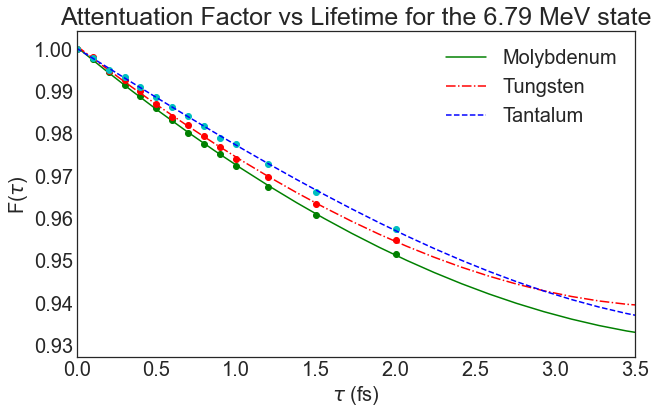
\includegraphics[width=\linewidth]{figures/attFacExample.png}
\caption{The calculated attenuation factors, $F(\tau)$, for the various experimental backings, as a function of the nuclear lifetime, $\tau$. This example of their relationship shows the various targets used in the measurement  and the response in the range of very short lifetimes, $\tau < 5$ fs, for the 6.79 MeV state in $^{15}$O. }
\label{fig: attFacExample}
\end{figure}



\section{Systematic errors and uncertainties}
\label{sec: systematicErrors}

This section details the instances and sources of systematic errors and uncertainties that arose in this treatment of the data and how they were managed.

\begin{enumerate}
\item In describing the SRIM software, Ziegler \textit{et al}.\ quoted the uncertainties in the programs stopping powers as 5\% \cite{Ziegler2010}. This was propagated through to an uncertainty in the initial energy of the recoiling ion paths as generated by SRIM for use in the MC simulation. This, ultimately, manifests in the distributions of $\gamma$ ray energies produced in the simulation and does not need to be otherwise included explicitly in this calculation. 
\item A significant difference between this procedure and other, previous methods for calculating the lifetimes is that this is not an analytical expression of the parameters and is only a numerical calculation. As a matter of fact, this is only a discrete calculation at values chosen across the relevant lifetime landscape. Therefore, these attenuation factors require an external fit to provide the final relationship. To minimize any artificial bias from the choice of simulated lifetimes, the lifetimes were chosen to range across the entire expected range of values and beyond to ensure that the relationship is robust in the relevant lifetime ranges. 
\item When considering the nominal angles of the detector placement in the measurement, it is critical that these be accurate to the target or they will introduce artificial changes in the Doppler shift relation. Put another way, if the target is not located at the axis of rotation for the detector, there will be an additional difference in the angles, causing inaccurate $F(\tau)$ determinations. To ensure that the target is at the axis of rotation for the detector, spectra were obtained at $\pm$ 90$\degree$. At both angles, $E_{\gamma}$ should be unshifted, since this angle is perpendicular to the motion of the recoiling nuclei. Therefore, the spectra at these angles should, and do, lie exactly on top of each other. This is presented in Fig.\ \ref{fig: pm90}. The agreement of these spectra demonstrates that the target was located at the center of the measurement apparatus and guarantees that the measured angles are accurate.

\begin{figure}
\thisfloatpagestyle{plain}
\centering
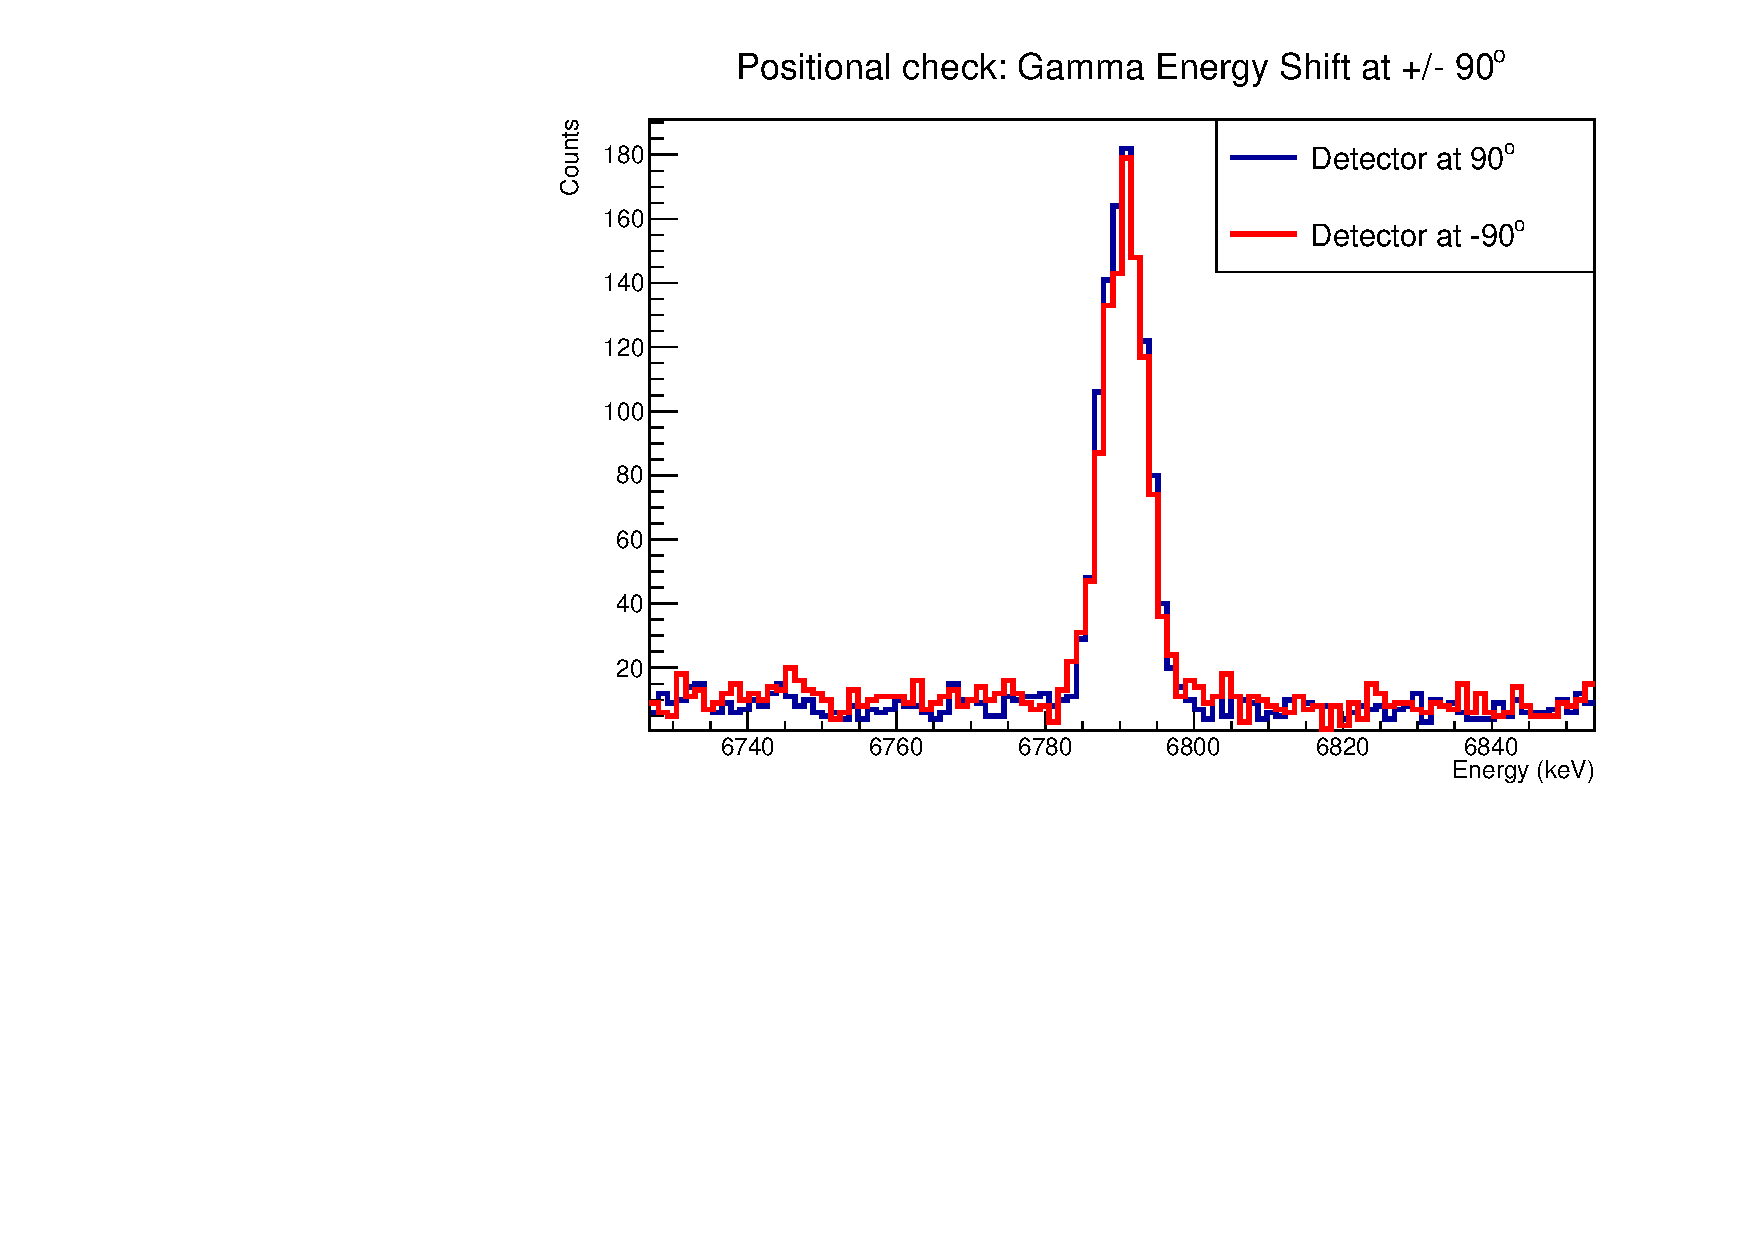
\includegraphics[width=\linewidth]{figures/pm90comparison.pdf}
\caption{Measured energy spectrum of the 6.79 MeV transition at $\pm$90$\degree$. At these two angles, the energy of the $\gamma$ ray is not Doppler shifted and so the fact that both spectra show perfect agreement indicates that there is no systematic effect in our measurement from inaccurate angular determination of the detector's positions.}
\label{fig: pm90}
\end{figure}


\item In fitting the peaks present in the spectra, the centroid, area, and width are extracted after removing a linear background contribution from the spectrum. The background was fit separately from the peak using regions surrounding the peak of interest to increase the fidelity of the background estimation. Fig.\ \ref{fig: bgfit} demonstrates this procedure. In this high-energy region of the spectrum, a linear background is a reasonable assumption, as the background always is quite small and peaks are typically well isolated from each other. 

\begin{figure}
\thisfloatpagestyle{plain}
\centering
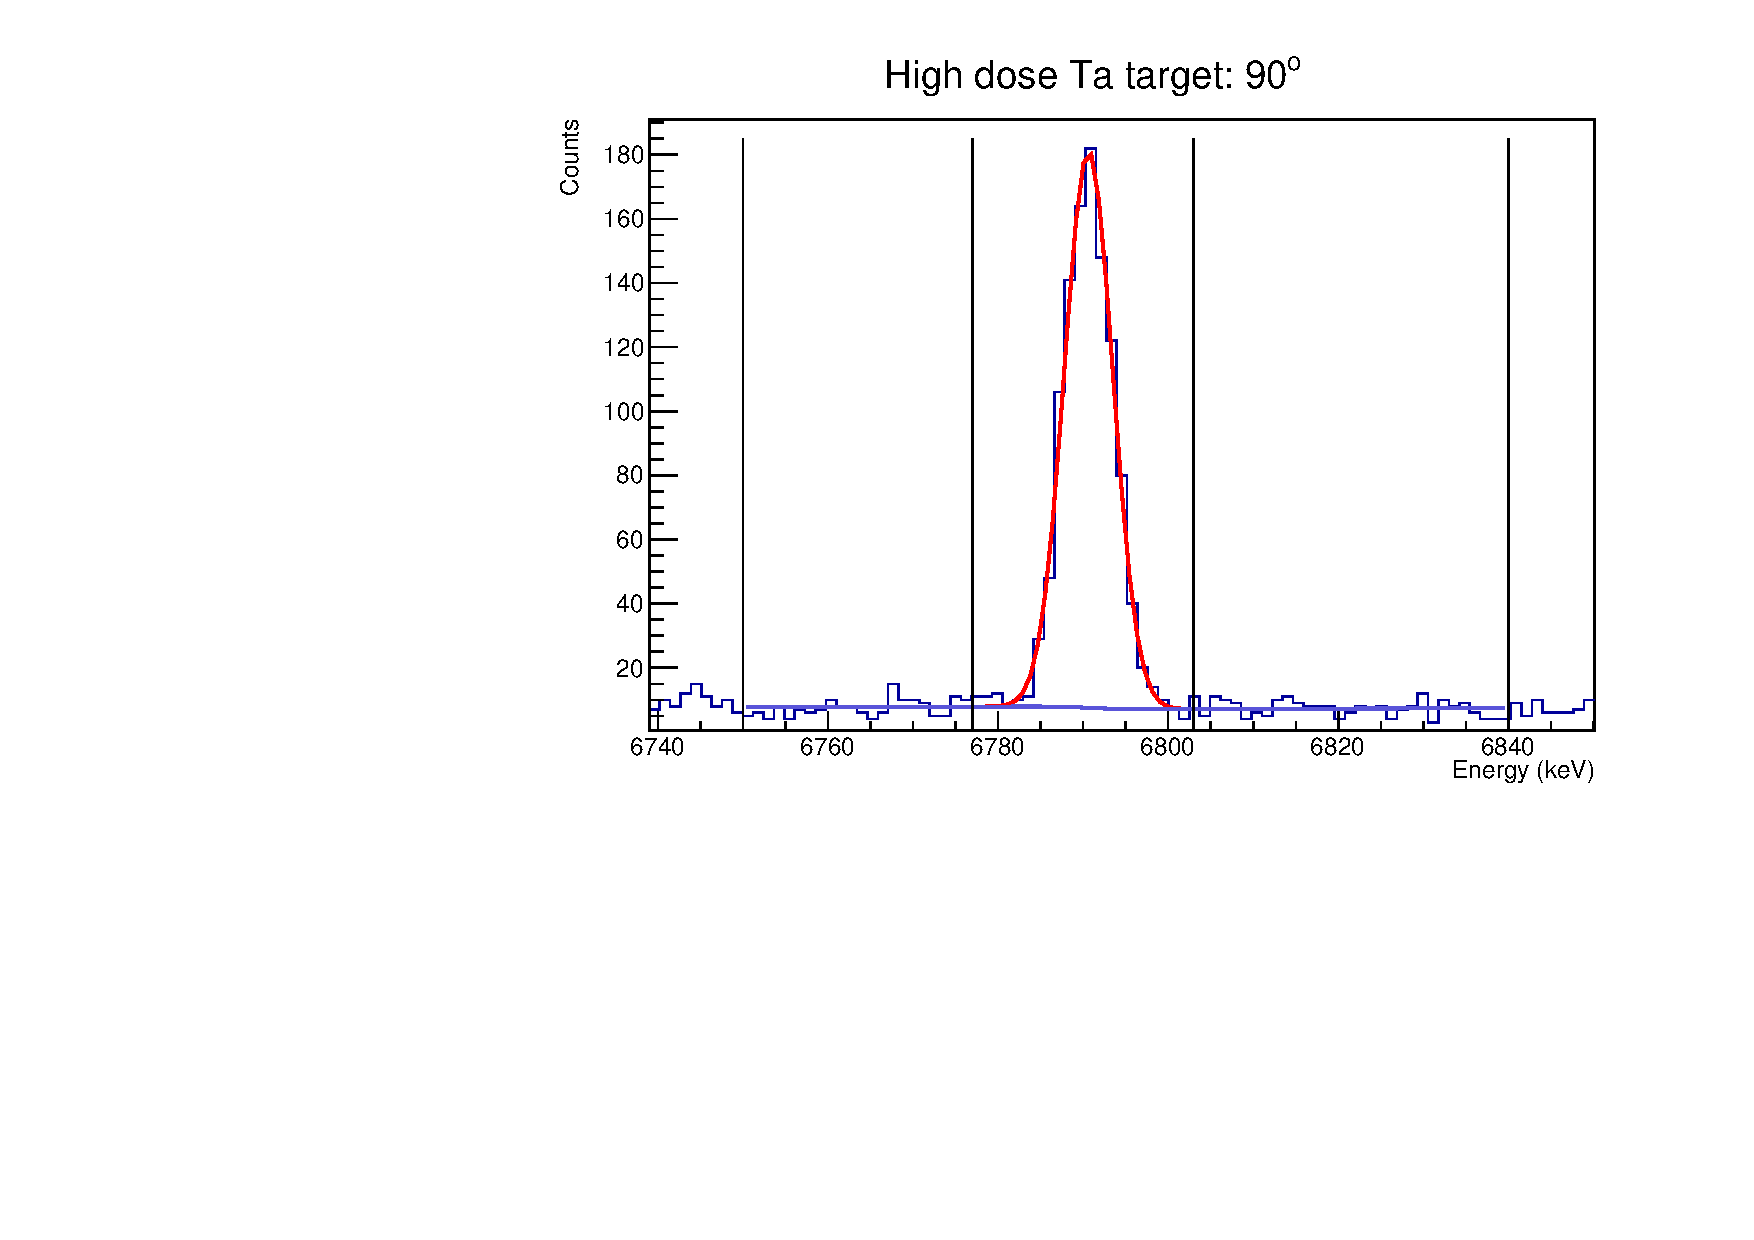
\includegraphics[width=0.7\linewidth]{figures/bgFit.pdf}
\caption{The stopped $\gamma$ ray peak as an example of the background subtraction method. The regions surrounding the peak of interest (marked by the black, vertical lines) are fit with a linear term to describe the background underneath the peak, which is fit separately with a Gaussian. }
\label{fig: bgfit}
\end{figure}

\item Due to experimental time constraints, the low dose implanted Ta target was only measured with two angles. Since two points define a line completely, the data give no measure of uncertainty. Therefore, this was ultimately excluded from subsequent analysis.
\item Compared to the cross section measurements, the number of $^{14}$N($p,\gamma)^{15}$O reactions that occur is not necessary for the lifetime determination, only the shift of the gamma's peak in the spectrum. As such, correcting the spectrum for efficiency or dead-time are unnecessary, as both effects only adjust the number of counts in a spectrum. Particularly when considering a small range of energies (like the 20 keV under a peak), efficiency effects are consistent across the peak range. Similarly, as dead-time effects are not energy dependent, they do not introduce any mis-shaping or artificial shifting of the peak.
%\item Orthogonal distance relation
\item The measurement uncertainties in the angle and centroid energy of the $\gamma$ peaks are represented as X and Y uncertainties, respectively, in evaluating the Doppler shift as function of angle. These are then propagated through a fit of the slope as the uncertainty on that fit parameter. As traditional least-squares fitting relies only on uncertainty in the Y position of data, these were fit with a method called Orthogonal Distance Regression (ODR), which incorporates point uncertainties in both the X and Y directions for the fit. Therefore, the slopes and uncertainties extracted by this ODR method have a higher fidelity compared with the traditional least-squares method. 
\end{enumerate}

\section{Lifetime of the 5.18 MeV state in $^{15}$O}
\label{sec: lifetime518}

The experimental Doppler shift of the $\gamma$ ray peaks for this decay can be seen in Fig.\ \ref{fig: shift518}. This figure displays the spectra for all of the measurements with different target materials and plots the spectra of different angular measurements together. This figure directly shows the shifting $\gamma$ ray peak for each of the angles measured in this work. Each of these were then fit with a Gaussian and underlying linear background, as described in Sec.\ \ref{sec: systematicErrors}, to determine their centroid and uncertainty. 


\begin{figure}
\thisfloatpagestyle{plain}
\centering
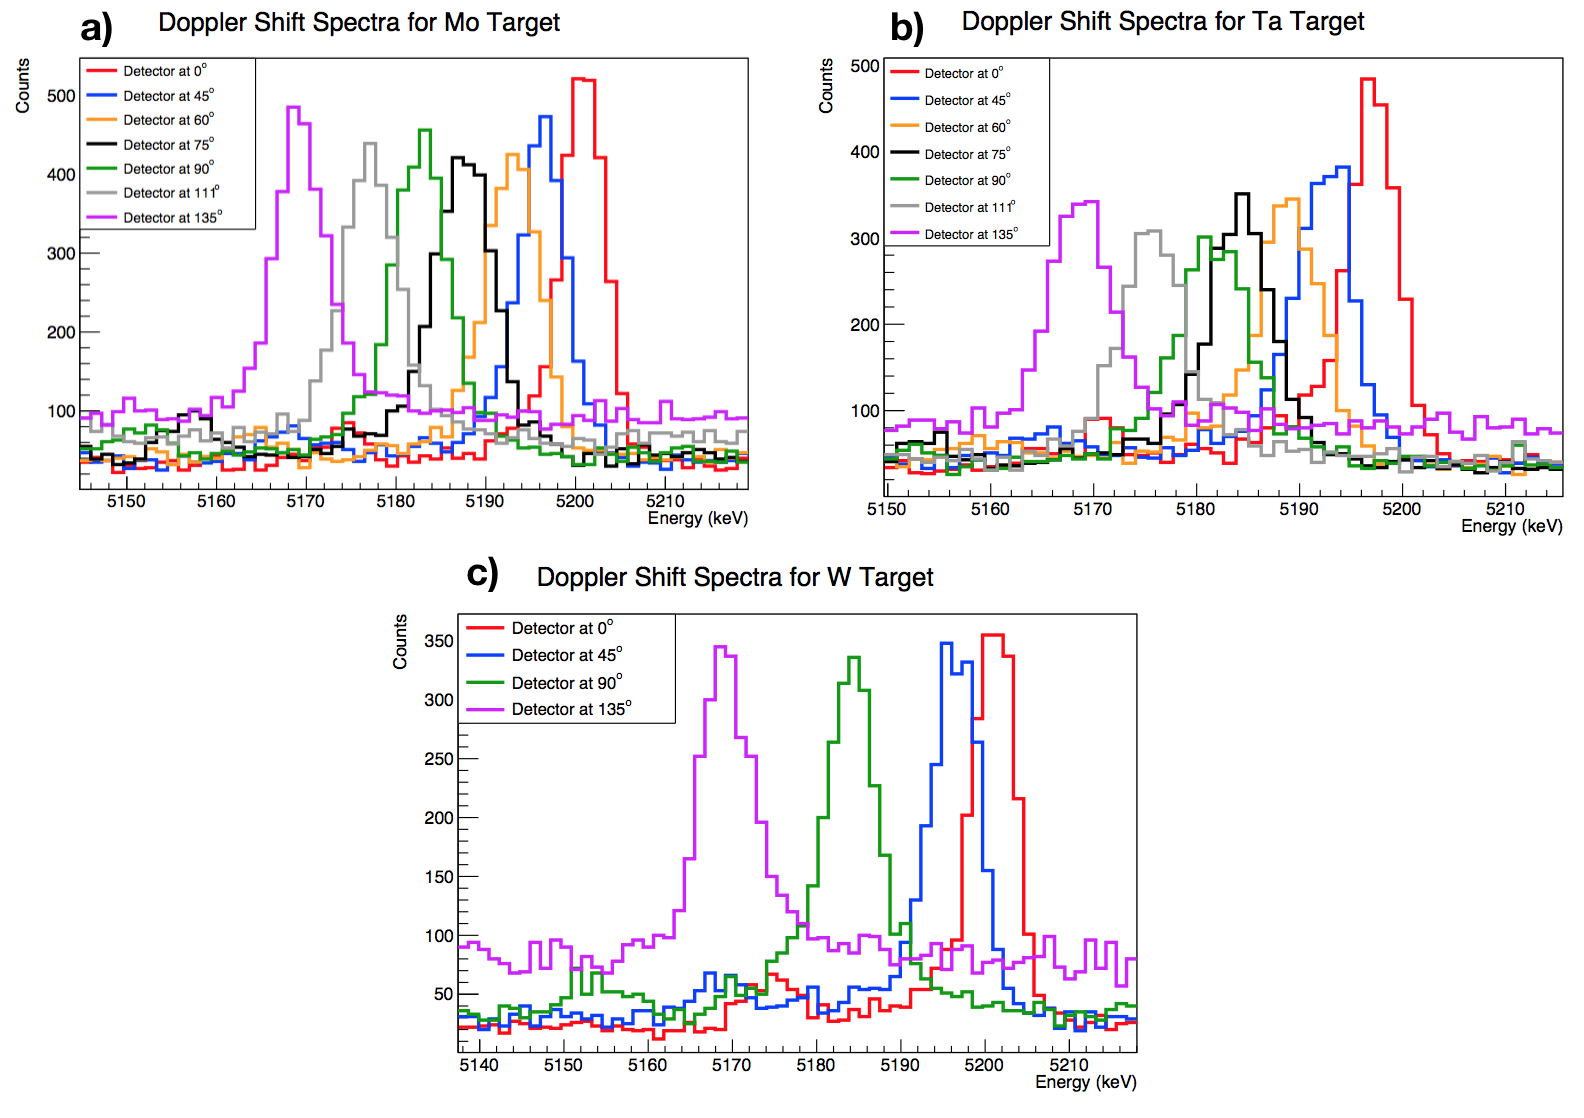
\includegraphics[width=0.6\linewidth]{figures/shifts518.png}
\caption{The Doppler shifted spectra taken during this measurement for the 5.18 MeV state. a) shows the spectra from the Mo implanted target, b) depicts the spectra from the Ta implanted target, and c) gives the spectra from the W implanted target.Within these, the Doppler shift boosting the energy of the $\gamma$ ray peak  with a change in angle can be clearly seen. }
\label{fig: shift518}
\end{figure}


With the measured energies of the $\gamma$-rays and their uncertainties, the relationship between the cosine of the measurement angle, $\cos(\theta)$, and the observed energies, $E_{\gamma}$, were determined for each of the target materials. This was achieved by fitting a straight line to the data with ODR, accounting for uncertainties in X and Y. Recall, the slope of this line is related to the experimentally measured attenuation factor, $F(\tau)$, which contains the lifetime information. These relationships are plotted in Fig.\ \ref{fig: doppler518} and their corresponding extracted $F(\tau)$ values are provided in Table \ref{table: afTau518}. The attenuation factor for this state with the Mo implanted target was $F(\tau)_{\text{Mo}} = 0.904 \pm 0.013$, $F(\tau)_{\text{Ta}} = 0.911 \pm 0.016$ with the Ta implanted target, and $F(\tau)_{\text{W}} = 0.912 \pm 0.015$ with the W implanted targets.


\begin{figure}
\thisfloatpagestyle{plain}
\centering
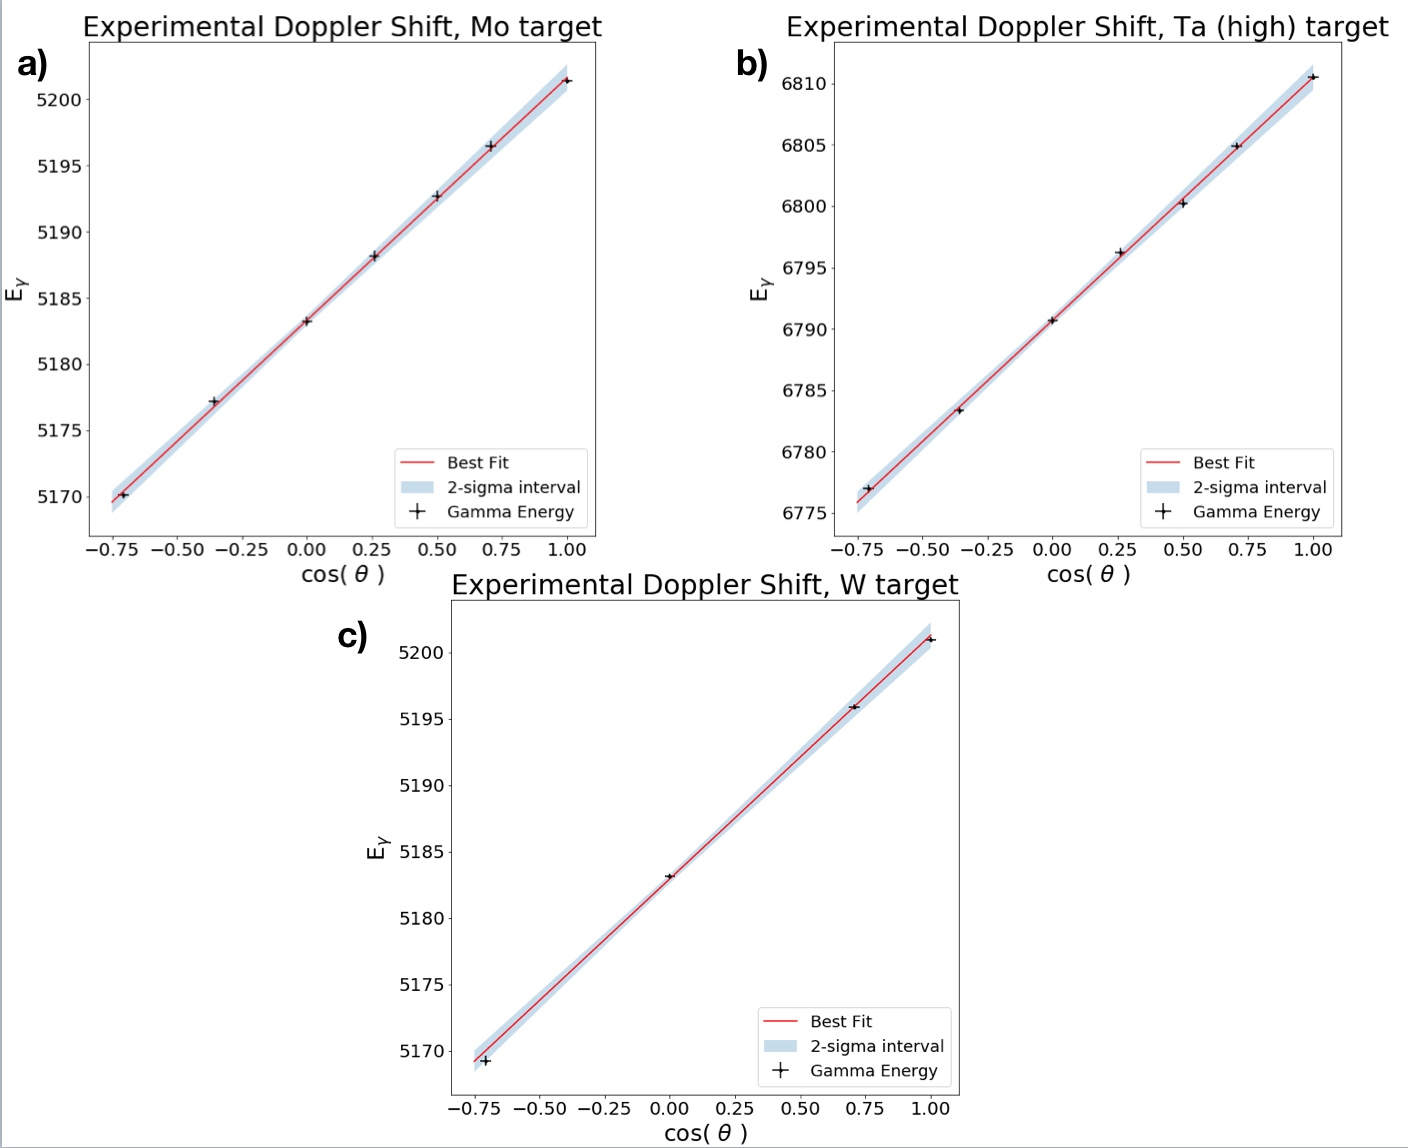
\includegraphics[width=\linewidth]{figures/doppler518.png}
\caption{The relationship between the measured angle, $\cos(\theta)$, and the measured $\gamma$ peak energy, $E_{\gamma}$ of the 5.18 MeV state for the a) Mo target, b) Ta target, and c) W target. The slopes, which contain the information about the attenuation factor, $F(\tau)$, and ultimately the lifetime, $\tau$, were determined with Orthogonal Distance Regression (see text for details). }
\label{fig: doppler518}
\end{figure}


\begin{table}[]
\thisfloatpagestyle{plain}
\caption{ATTENUATION FACTORS AND LIFETIMES OF THE 5.18 MeV STATE MEASURED IN THIS WORK}
\centering
\begin{threeparttable}
\begin{tabular}{@{}lllll@{}}
\toprule
                   & Mo Target  & Ta Target & W Target & Weighted Average \\ \midrule
$F(\tau)_{5.18}$   & $9.040 \pm 0.013$     & $0.911 \pm 0.016$   & $9.120 \pm 0.015$   &                  \\
$\tau_{5.18}$ (fs) & $7.1^{+4.8}_{-2.3}$ & $7.1 \pm 5.5$       & $8.0 \pm 6.7$      & $7.3 \pm 3.2$    \\ \bottomrule
\end{tabular}
\begin{tablenotes}
\small 
\item A summary of the attenuation factors and lifetime measurements for the 5.18 MeV state in $\ce{^{15}O}$. All measurements are listed with their corresponding target material and the weighed average for the lifetime is also provided. To note, it is not possible to take a weighted average of the attenuation factor because the response of the attenuation factor to lifetime is highly dependent on the target material, so only an average of the extracted lifetimes are accurate.
\end{tablenotes}
\end{threeparttable}
\label{table: afTau518}
\end{table}

For this state, the attenuation factor curves, which relates the nuclear lifetime to the $F(\tau)$ values, are shown for each target material in Fig.\ \ref{fig: attFacs518}. It is through this relationship that the measured lifetimes are determined. From the measured attenuation factors, the measured lifetimes for this state are $\tau_{\text{Mo}} = 7.1^{+4.8}_{-2.3}$ fs with the Mo implanted target, $\tau_{\text{Ta}} = 7.1 \pm 5.5$ fs with the Ta implanted target, and $\tau_{\text{W}} = 8.0 \pm 6.7$ fs from the W implanted target. The weighted average of these measurements is $\overline{\tau} = 7.3 \pm 3.2$ fs. These values, as well as existing literature measurements of the lifetime of this state, are presented in Fig.\ \ref{fig: lifetimes518} and are summarized in Table \ref{table: afTau518}. As can be seen, these new measurements have significantly higher uncertainties than previous measurements of this state's lifetime. This comes primarily from the response of the attenuation factor to lifetime in this range. As can be seen in Fig.\ \ref{fig: attFacs518}, this region of lifetimes has a relatively flat response. Due to this, even a small error of 1-2\% in the $F(\tau)$ compounds into a larger uncertainty in the measured lifetime. Ultimately, this means that we have a less precise value than those of Refs.\ \cite{Bertone2001, Schurmann2008, Gill1968} but we still show good agreement with all three of those reported values.


\begin{figure}
\thisfloatpagestyle{plain}
\centering
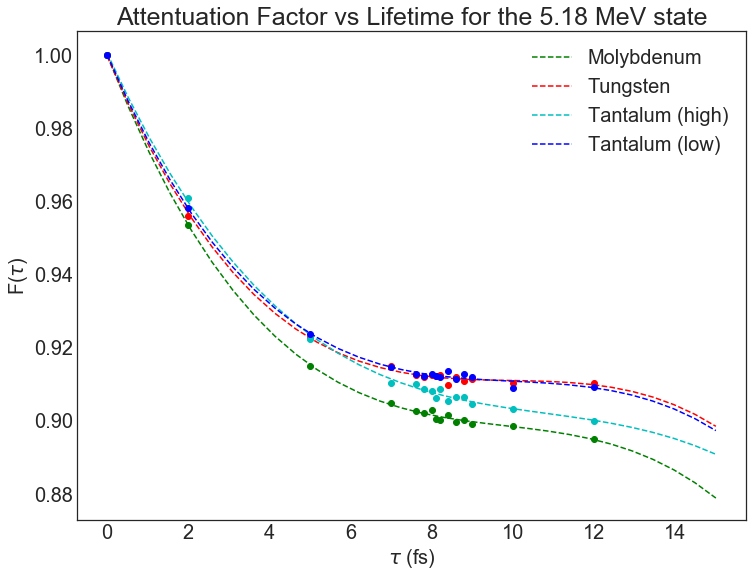
\includegraphics[width=\linewidth]{figures/attFac518.png}
\caption{The calculated attenuation factors, $F(\tau)$, for the various experimental backings, as a function of the nuclear lifetime, $\tau$, for the 5.18 MeV state in $^{15}$O. While the low dose Ta target is included in the calculation, it was excluded for a lifetime determination (see Section \ref{sec: systematicErrors} for details). }
\label{fig: attFacs518}
\end{figure}


\begin{figure}
\thisfloatpagestyle{plain}
\centering
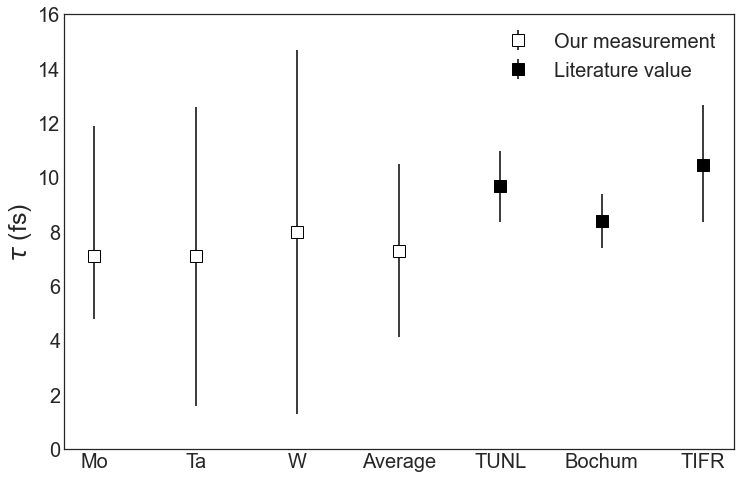
\includegraphics[width=\linewidth]{figures/lifetimes518.png}
\caption{Measured lifetimes and the weighted average lifetime of the 5.18 MeV state in $^{15}$O determined in this work (green box) alongside literature values. The TUNL measurement is Ref.\ \cite{Bertone2001} and the Bochum measurement is Ref.\ \cite{Schurmann2008}. On the whole, our measured values are less precise than the other literature values, but agree well with those same reports.}
\label{fig: lifetimes518}
\end{figure}



\section{Lifetime of the 6.17 MeV state in $^{15}$O}
\label{sec: lifetime617}


The experimental Doppler shift of the $\gamma$ ray peaks for this decay can be seen in Fig.\ \ref{fig: shift617}. This figure displays the spectra for all of the measurements with different target materials and plots the spectra of different angular measurements together. This figure directly shows the shifting $\gamma$ ray peak for each of the angles measured in this work. Each of these were then fit with a Gaussian and underlying linear background, as described in Sec.\ \ref{sec: systematicErrors}, to determine their centroid and uncertainty. 


\begin{figure}
\thisfloatpagestyle{plain}
\centering
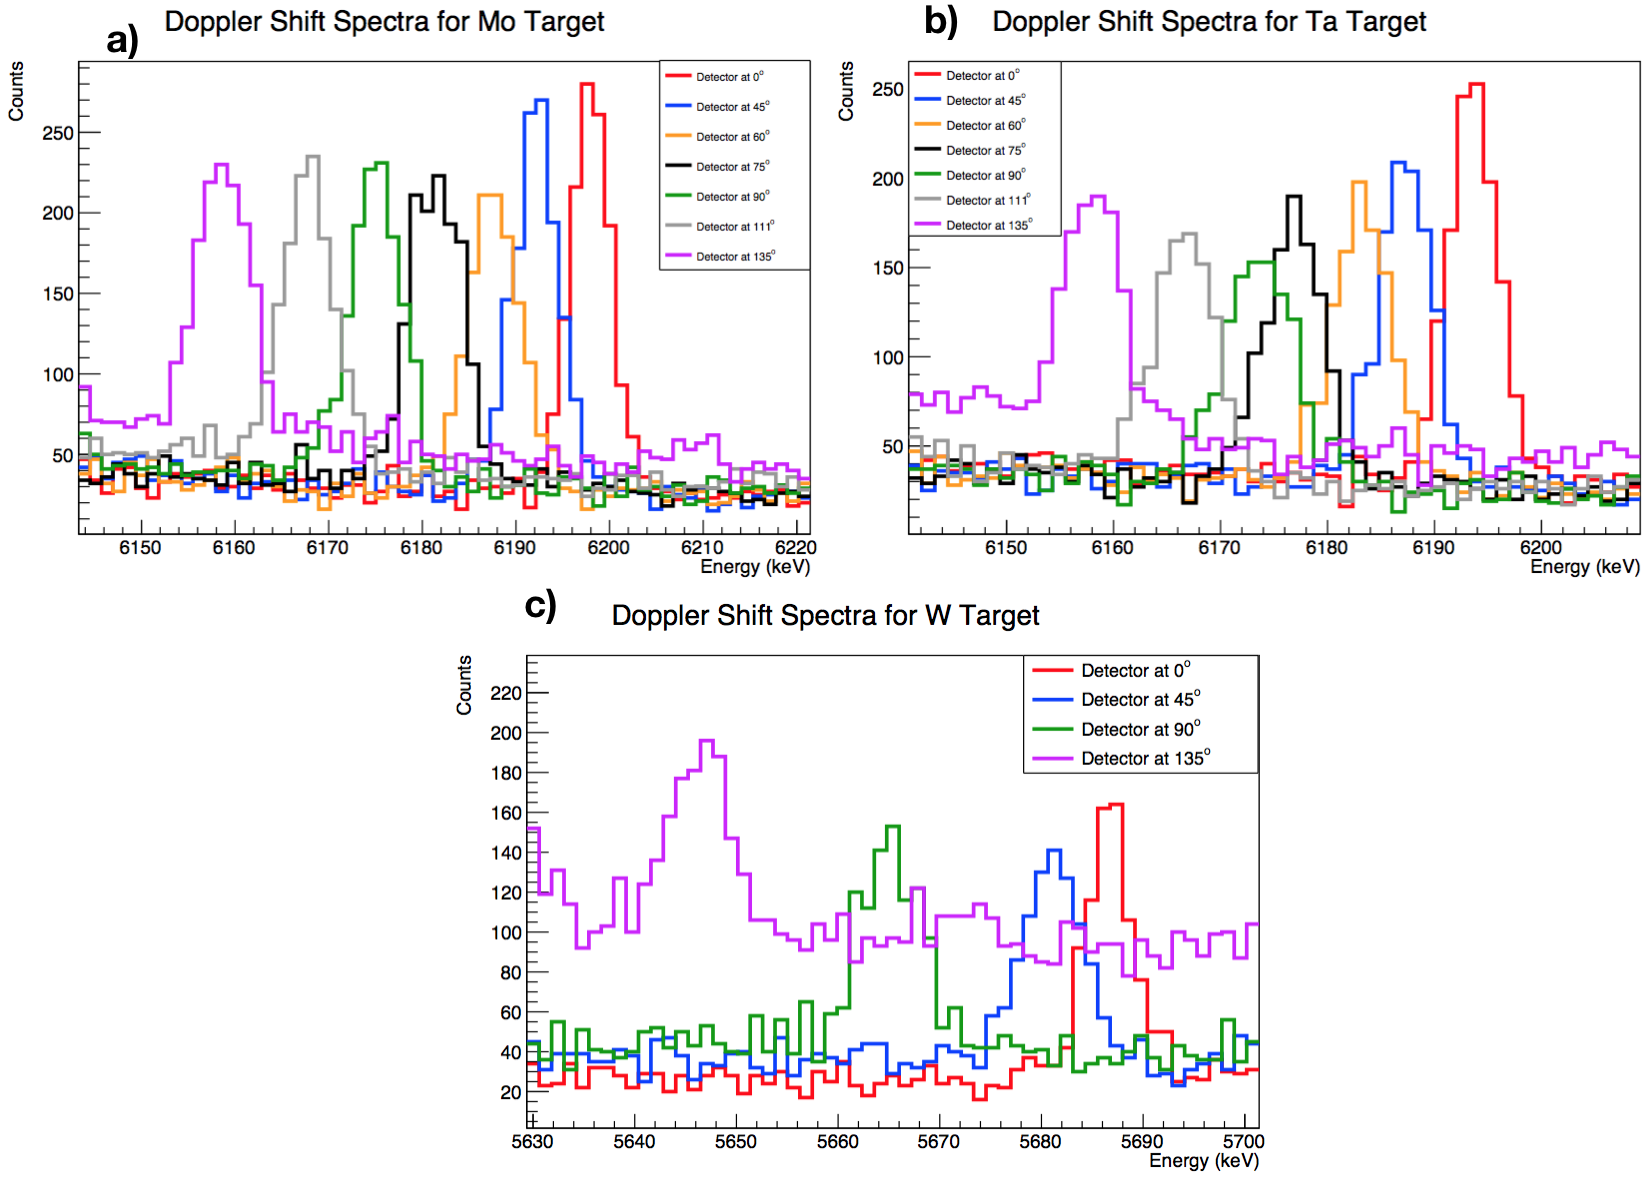
\includegraphics[width=0.6\linewidth]{figures/shifts617.png}
\caption{The Doppler shifted spectra taken during this measurement for the 6.17 MeV state. a) shows the spectra from the Mo implanted target, b) depicts the spectra from the Ta implanted target, and c) gives the spectra from the W implanted target.Within these, the Doppler shift boosting the energy of the $\gamma$ ray peak  with a change in angle can be clearly seen. }
\label{fig: shift617}
\end{figure}


With the measured energies of the $\gamma$-rays and their uncertainties, the relationship between the cosine of the measurement angle, $\cos(\theta)$, and the observed energies, $E_{\gamma}$, were determined for each of the target materials. This was achieved by fitting a straight line to the data with ODR, accounting for uncertainties in X and Y. Recall, the slope of this line is related to the experimentally measured attenuation factor, $F(\tau)$, which contains the lifetime information. These relationships are plotted in Fig.\ \ref{fig: doppler617} and their corresponding extracted $F(\tau)$ values are provided in Table \ref{table: afTau617}. The attenuation factor for this state with the Mo implanted target was $F(\tau)_{\text{Mo}} = 0.992 \pm 0.014$, $F(\tau)_{\text{Ta}} = 0.976 \pm 0.017$ with the Ta implanted target, and $F(\tau)_{\text{W}} = 0.988 \pm 0.016$ with the W implanted targets.


\begin{figure}
\thisfloatpagestyle{plain}
\centering
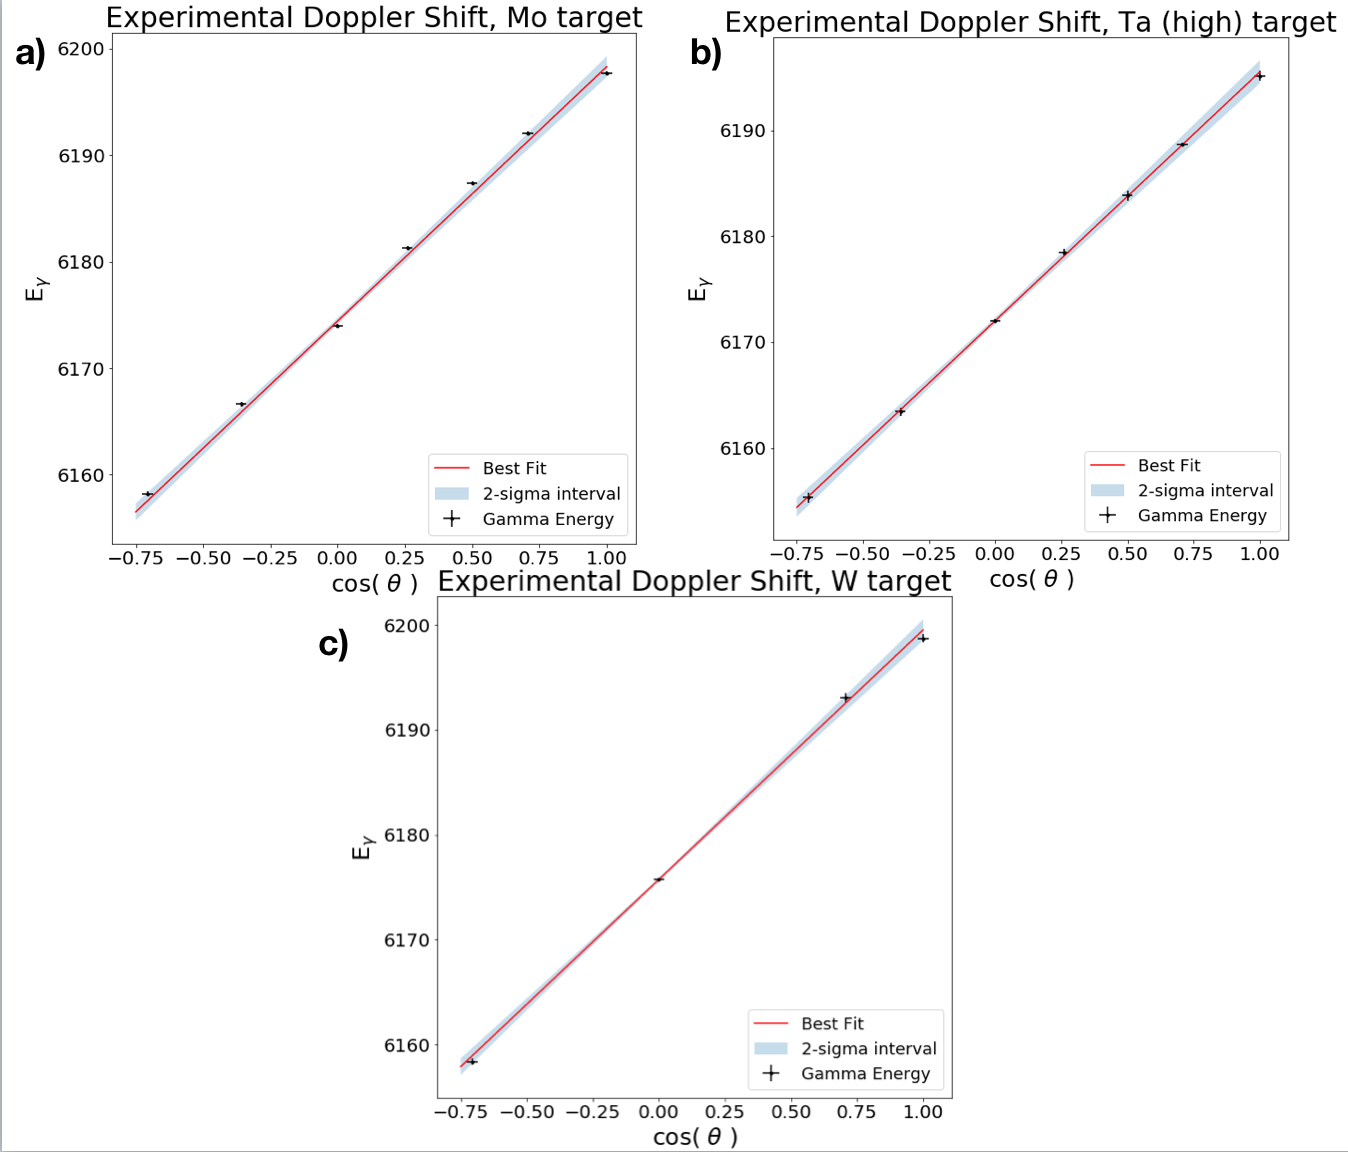
\includegraphics[width=\linewidth]{figures/doppler617.png}
\caption{The relationship between the measured angle, $\cos(\theta)$, and the measured $\gamma$ peak energy, $E_{\gamma}$ of the 6.17 MeV state for the a) Mo target, b) Ta target, and c) W target. The slopes, which contain the information about the attenuation factor, $F(\tau)$, and ultimately the lifetime, $\tau$, were determined with Orthogonal Distance Regression (see text for details). }
\label{fig: doppler617}
\end{figure}

\begin{table}[]
\thisfloatpagestyle{plain}
\caption{ATTENUATION FACTORS AND LIFETIMES OF THE 6.17 MeV STATE MEASURED IN THIS WORK}
\centering
\begin{threeparttable}
\begin{tabular}{@{}lllll@{}}
\toprule
                   & Mo Target & Ta Target & W Target  & Weighted Average \\ \midrule
$F(\tau)_{6.17}$   & $0.992 \pm 0.014$   & $0.976 \pm 0.017$   & $0.988 \pm 0.016$   &                  \\
$\tau_{6.17}$ (fs) & $0.4^{+0.7}_{-0.4}$ & $1.4 \pm 1.0$       & $0.6^{+0.9}_{-0.6}$ & $0.7 \pm 0.5$    \\ \bottomrule
\end{tabular}
\begin{tablenotes}
\small 
\item A summary of the attenuation factor and lifetime measurements for the 6.17 MeV state in $\ce{^{15}O}$. All measurements are listed with their corresponding target material and their weighed average is provided. To note, it is not possible to take a weighted average of the attenuation factor because the response of the attenuation factor to lifetime is highly dependent on the target material, so only an average of the extracted lifetimes are accurate.
\end{tablenotes}
\end{threeparttable}
\label{table: afTau617}
\end{table}

For this state, the attenuation factor curves, which relates the nuclear lifetime to the $F(\tau)$ values, are shown for each target material in Fig.\ \ref{fig: attFacs617}. It is through this relationship that the measured lifetimes are determined. From the measured attenuation factors, the measured lifetimes for this state are $\tau_{\text{Mo}} = 0.4^{+0.7}_{-0.4}$ fs with the Mo implanted target, $\tau_{\text{Ta}} = 1.4 \pm 1.0$ fs with the Ta implanted target, and $\tau_{\text{W}} = 0.6^{+0.9}_{-0.6}$ fs from the W implanted target. The weighted average of these measurements is $\overline{\tau} = 0.7 \pm 0.5$ fs. These values, as well as existing literature measurements of the lifetime of this state, are presented in Fig.\ \ref{fig: lifetimes617} and are summarized in Table \ref{table: afTau617}. For this state, we report a significantly more precise value than those of Refs.\ \cite{Bertone2001, Schurmann2008, Galinski2014}. We show only a minimal agreement within uncertainty to the TUNL measurement \cite{Bertone2001}. Our reported value is engulfed entirely within the upper bound placed by \cite{Galinski2014} and lies just within the edge of the upper bound reported in \cite{Schurmann2008}, with a significant overlap on our uncertainty range. Our value, thus, aligns most agreeably with that of Sch{\"u}rmann \textit{et al.} \cite{Schurmann2008}.


\begin{figure}
\thisfloatpagestyle{plain}
\centering
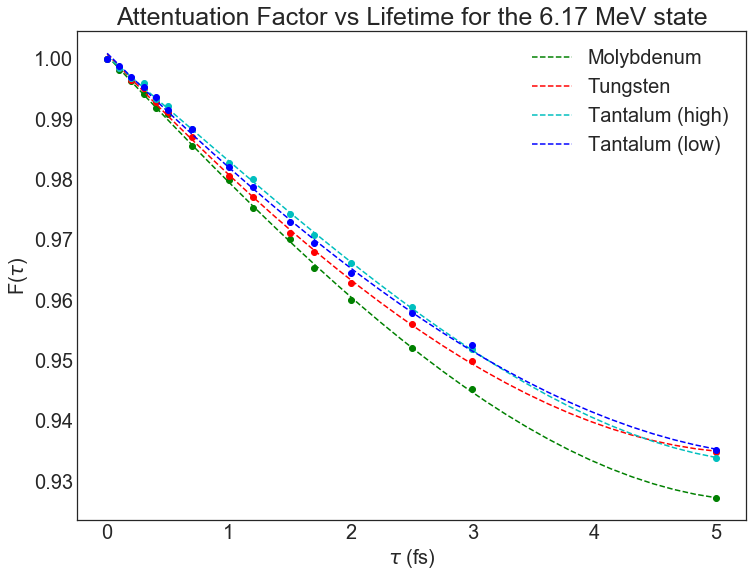
\includegraphics[width=\linewidth]{figures/attFac617.png}
\caption{The calculated attenuation factors, $F(\tau)$, for the various experimental backings, as a function of the nuclear lifetime, $\tau$, for the 6.17 MeV state in $^{15}$O. While the low dose Ta target is included in the calculation, it was excluded for a lifetime determination (see Section \ref{sec: systematicErrors} for details).}
\label{fig: attFacs617}
\end{figure}


\begin{figure}
\thisfloatpagestyle{plain}
\centering
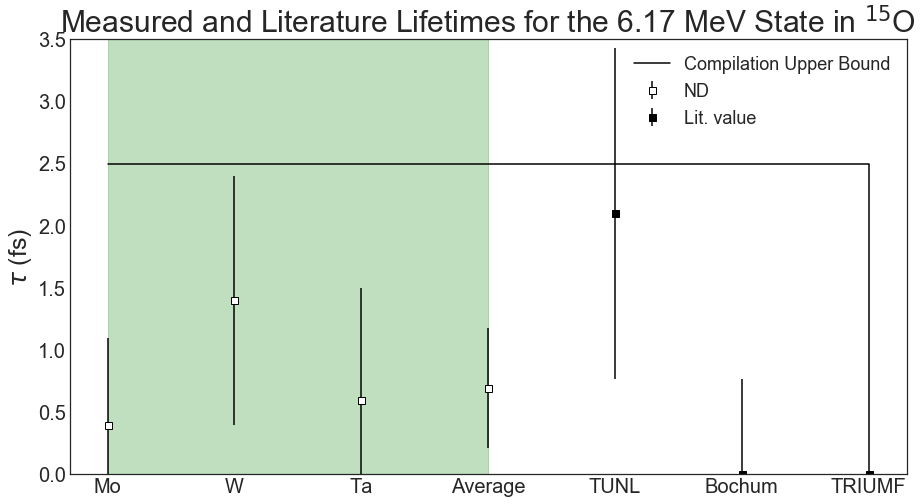
\includegraphics[width=\linewidth]{figures/lifetimes617.png}
\caption{Measured lifetimes and the weighted average lifetime of the 5.18 MeV state in $^{15}$O determined in this work (green box) alongside literature values. The TUNL measurement is Ref.\ \cite{Bertone2001}, the Bochum measurement is Ref.\ \cite{Schurmann2008}, and the TRIUMF measurement is Ref.\ \cite{Galinski2014}. Here, our results are more precise and agree very well with the measurements of Sch{\"u}rmann \textit{et al.} \cite{Schurmann2008} and Galinski \textit{et al.} \cite{Galinski2014}, while also showing weak agreement with the measurement reported by Ref.\ \cite{Bertone2001}. }
\label{fig: lifetimes617}
\end{figure}



\section{Lifetime of the 6.79 MeV state in $^{15}$O}
\label{sec: lifetime679}


The experimental Doppler shift of the $\gamma$ ray peaks for this decay can be seen in Fig.\ \ref{fig: shift679}. This figure displays the spectra for all of the measurements with different target materials and plots the spectra of different angular measurements together. This figure directly shows the shifting $\gamma$ ray peak for each of the angles measured in this work. Each of these were then fit with a Gaussian and underlying linear background, as described in Sec.\ \ref{sec: systematicErrors}, to determine their centroid and uncertainty. 


\begin{figure}
\thisfloatpagestyle{plain}
\centering
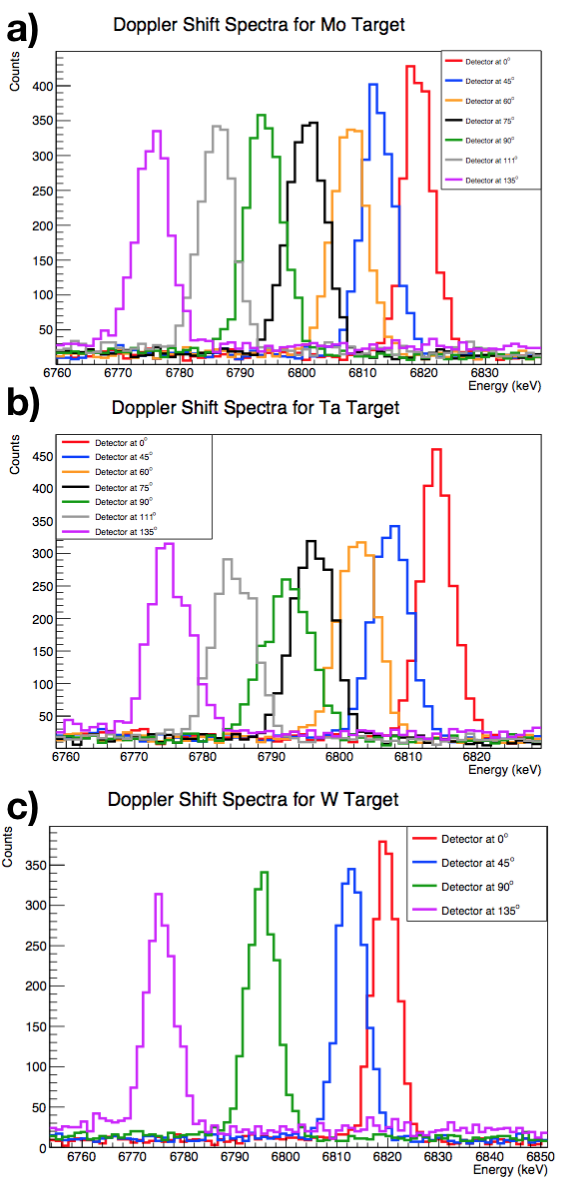
\includegraphics[width=0.6\linewidth]{figures/shifts679.png}
\caption{The Doppler shifted spectra taken during this measurement for the 6.79 MeV state. a) shows the spectra from the Mo implanted target, b) depicts the spectra from the Ta implanted target, and c) gives the spectra from the W implanted target.Within these, the Doppler shift boosting the energy of the $\gamma$ ray peak  with a change in angle can be clearly seen. }
\label{fig: shift679}
\end{figure}


With the measured energies of the $\gamma$-rays and their uncertainties, the relationship between the cosine of the measurement angle, $\cos(\theta)$, and the observed energies, $E_{\gamma}$, were determined for each of the target materials. This was achieved by fitting a straight line to the data with ODR, accounting for uncertainties in X and Y. Recall, the slope of this line is related to the experimentally measured attenuation factor, $F(\tau)$, which contains the lifetime information. These relationships are plotted in Fig.\ \ref{fig: doppler679} and their corresponding extracted $F(\tau)$ values are provided in Table \ref{table: afTau679}. The attenuation factor for this state with the Mo implanted target was $F(\tau)_{\text{Mo}} =0.995 \pm 0.019$, $F(\tau)_{\text{Ta}} = 0.983 \pm 0.019$ with the Ta implanted target, and $F(\tau)_{\text{W}} = 0.978 \pm 0.015$ with the W implanted targets.


\begin{figure}
\thisfloatpagestyle{plain}
\centering
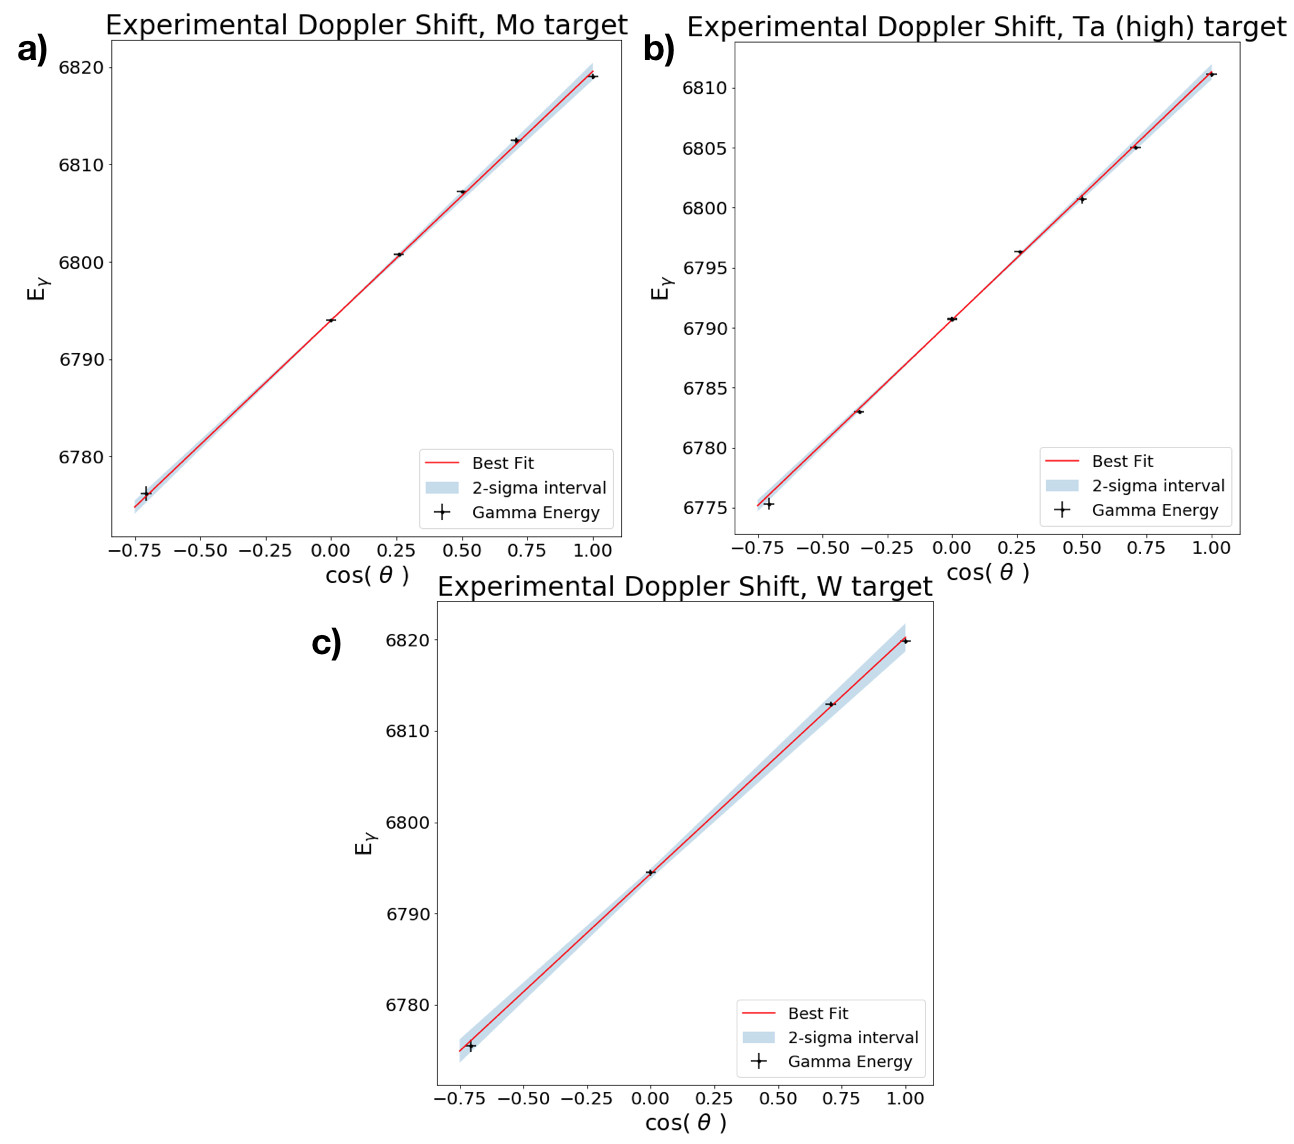
\includegraphics[width=\linewidth]{figures/doppler679.png}
\caption{The relationship between the measured angle, $\cos(\theta)$, and the measured $\gamma$ peak energy, $E_{\gamma}$ of the 6.79 MeV state for the a) Mo target, b) Ta target, and c) W target. The slopes, which contain the information about the attenuation factor, $F(\tau)$, and ultimately the lifetime, $\tau$, were determined with Orthogonal Distance Regression (see text for details). }
\label{fig: doppler679}
\end{figure}

\begin{table}[]
\thisfloatpagestyle{plain}
\caption{ATTENUATION FACTORS AND LIFETIMES OF THE 6.79 MeV STATE MEASURED IN THIS WORK}
\centering
\begin{threeparttable}
\begin{tabular}{@{}lllll@{}}
\toprule
                   & Mo Target & Ta Target & W Target & Weighted Average \\ \midrule
$F(\tau)_{6.79}$   & $0.995 \pm 0.019$   & $ 0.983 \pm 0.019$  & $0.978 \pm 0.015$  &                  \\
$\tau_{6.79}$ (fs) & $0.2^{+0.7}_{-0.2}$ & $0.7^{+0.9}_{-0.7}$ & $0.9 \pm 0.6$      & $0.6 \pm 0.4$    \\ \bottomrule
\end{tabular}
\begin{tablenotes}
\small 
\item A summary of the attenuation factor and lifetime measurements for the 6.79 MeV state in $\ce{^{15}O}$. All measurements are listed with their corresponding target material and their weighed average is provided. To note, it is not possible to take a weighted average of the attenuation factor because the response of the attenuation factor to lifetime is highly dependent on the target material, so only an average of the extracted lifetimes are accurate.
\end{tablenotes}
\end{threeparttable}
\label{table: afTau679}
\end{table}


For this state, the attenuation factor curves, which relates the nuclear lifetime to the $F(\tau)$ values, are shown for each target material in Fig.\ \ref{fig: attFacs679}. It is through this relationship that the measured lifetimes are determined. From the measured attenuation factors, the measured lifetimes for this state are $\tau_{\text{Mo}} = 0.2^{+0.7}_{-0.2}$ fs with the Mo implanted target, $\tau_{\text{Ta}} = 0.7^{+0.9}_{-0.7}$ fs with the Ta implanted target, and $\tau_{\text{W}} = 0.9 \pm 0.6$ fs from the W implanted target. The weighted average of these measurements is $\overline{\tau} = 0.6 \pm 0.4$ fs. These values, as well as existing literature measurements of the lifetime of this state, are presented in Fig.\ \ref{fig: lifetimes679} and are summarized in Table \ref{table: afTau679}. For this state, as with the 6.17 MeV state, we obtain the most precise measured value. In another similarity to the 6.17 MeV state, our individual measurements and weighted average all lie on the edge of the range reported by Bertone \textit{et al.} \cite{Bertone2001}, while they agree much more concretely with those measurements reported in Refs.\ \cite{Schurmann2008, Galinski2014, Michelagnoli2013}. 


\begin{figure}
\thisfloatpagestyle{plain}
\centering
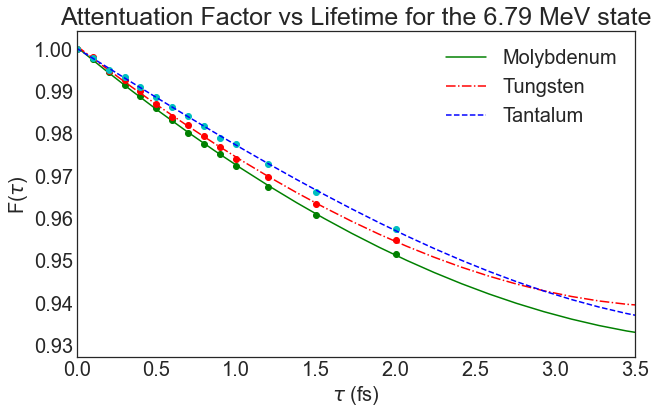
\includegraphics[width=\linewidth]{figures/attFac679.png}
\caption{The calculated attenuation factors, $F(\tau)$, for the various experimental backings, as a function of the nuclear lifetime, $\tau$, for the 6.79 MeV state in $^{15}$O. While the low dose Ta target is included in the calculation, it was excluded for a lifetime determination (see Section \ref{sec: systematicErrors} for details). Our measurements of this state provide the most precise lifetime determination. Similar to our measurement of the 6.17 MeV state, the individually measured points as well as their weighted average agree well with the results from Sch{\"u}rmann \textit{et al.} \cite{Schurmann2008} and Galinski \textit{et al.} \cite{Galinski2014} and overlapping, albeit less well, with Ref.\ \cite{Bertone2001}.}
\label{fig: attFacs679}
\end{figure}


\begin{figure}
\thisfloatpagestyle{plain}
\centering
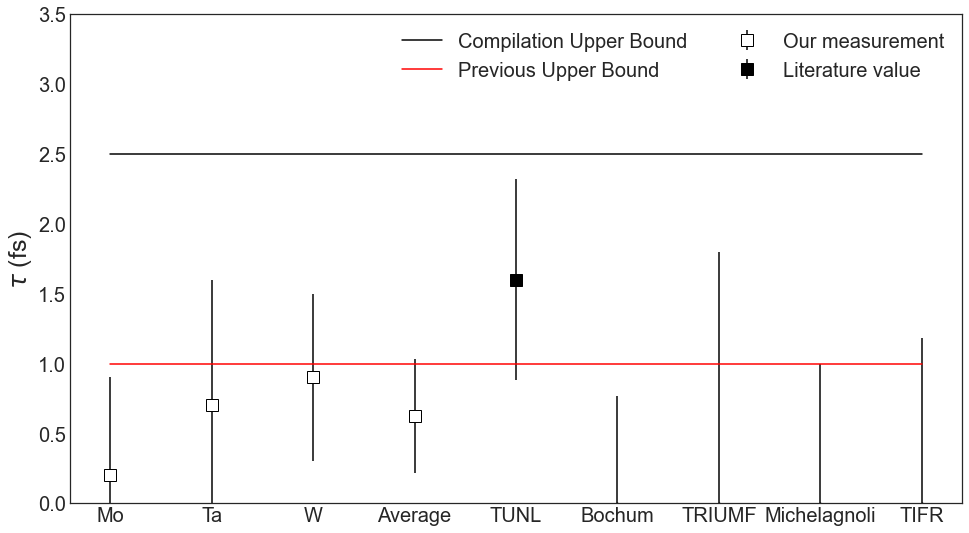
\includegraphics[width=\linewidth]{figures/lifetimes679.png}
\caption{Measured lifetimes and the weighted average lifetime of the 5.18 MeV state in $^{15}$O determined in this work (green box) alongside literature values. The TUNL measurement is Ref.\ \cite{Bertone2001}, the Bochum measurement is Ref.\ \cite{Schurmann2008}, the TRIUMF measurement is Ref.\ \cite{Galinski2014}, and the Michelagnoli measurement comes from Ref.\ \cite{Michelagnoli2013}. }
\label{fig: lifetimes679}
\end{figure}


\textbf{GIVE A SUMMARY. WE FOUND SOME GOOD STUFF. SUMMARY TABLE OF ALL OF THE DATA (COPIED FROM PAPER).}



% % uncomment the following lines,
% if using chapter-wise bibliography
%
% \bibliographystyle{ndnatbib}
% \bibliography{example}
